\chapter{Traction System}

\section{Introduction}
The traction system of the Hyperloop pod plays a pivotal role in ensuring the efficient transmission of power to the ground, facilitating the acceleration, and maintaining high-speed stability. This system is intricately designed to optimize the pod's grip and minimize slippage, particularly during high-speed operations and in varying track conditions. 

Key considerations for the traction system include the selection of materials and technologies that maximize frictional force while minimizing wear and energy loss. Additionally, the system must be robust enough to handle the dynamic loads and stresses encountered during rapid acceleration, sustained high-speed travel, and deceleration phases. 

In this section, we will delve into the specifics of the traction system, exploring its components, design considerations, and the integration with the overall pod architecture. The focus will be on ensuring that the system contributes to the overall efficiency, safety, and performance of the Hyperloop pod, aligning with the project's goals of high-speed and sustainable transportation.


\section{Propulsion}

\subsection{Overview}

To accelerate our Hyperloopod we use our EMRAX 188 electric motor from last season. This delivers an output of 60 kW under high voltage and a maximum torque of 100 Nm. This torque gets transferred to a right-angle gearbox and from there is slid to the drive wheels via cardan joints.

\subsubsection{Concept}
The main goal of this system is to accelerate our pod with an acceleration of \(5 \, \text{m/s}^2\). Since the given \(100 \, \text{Nm}\) are not sufficient under an estimated total weight of \(250 \, \text{kg}\), the drivetrain requires a gear ratio. Since an angular gearbox is installed anyway, it is easy to implement this criterion there. In order to maintain a relatively high top speed of the pod, this transmission ratio should be as close as possible. According to the formula
\[
T_{\text{required}} = \frac{{(m \cdot a + \frac{1}{2} \cdot \rho_{\text{air}} \cdot C_w \cdot A_{\text{Aeroshell}} \cdot v^2 + m \cdot g \cdot \cos(\Theta)) \cdot r}}{{\eta}}
\]
we know that we require at least around \(170 \, \text{Nm}\) of torque to achieve this amount of acceleration. While the pod weight of \(250 \, \text{kg}\) is only an estimate at the time of system design and we are always keen to get such complex parts from our partners, we opted for a \(2:1\) ratio of a Mädler gearbox. With this gear ratio, a respectable top speed of \(113 \, \text{km/h}\) is still possible. This is absolutely sufficient for our prototype, as we are still sticking to our basic idea: For low speeds and accelerations, we drive our hyperloop pod with a conventional wheel drive and for everything above that, the pod will hover with a linear induction motor which will be added in future prototypes. We believe that we can achieve an increase in efficiency in this way as permanent levitation is not necessary.

The transmitted torque must now be directed to the drive wheels in such a way that it is still possible to ensure a working suspension. For this, we use universal joints on both sides of the centered bevel gear. These also come from our partner Mädler and are connected to the bevel gear using in-house produced adapter shafts and feather keys. To finally connect the other ends of the shaft joints to the wheel, only one last shaft is missing. This is also fitted with a keyway on the joint side and a bolt circle on a flange on the wheel side. Now that the wheels are supplied with power, it is important to create sufficient rolling friction. To achieve this, Continental provides us with a rubber coating for our wheels. \\
Of course, this all has to be mounted into the chassis. For this, we use three different types of brackets beside the knuckles, where the wheelshafts are mounted: one for the motor, one for the motorshaft and two of the same kind, which carry everything between the shaft joints.

\subsubsection{Size, Components, and Appearance}

\autoref{table:components}
\begin{table}[ht]
\centering
\begin{adjustbox}{width=\textwidth}
\begin{tabular}{|>{\bfseries}m{2.5cm}|m{1.4cm}|m{1.7cm}|m{2.9cm}|m{2.2cm}|}
\hline
Component & Number & Mass [kg] & Size [mm] &  In-house/ outsourced \\
\hline
Motor & x1 & 7 & \(188 \times 188 \times 112\) &   Bought \\
Motorshaft & x1 & 0.4 & \(170 \times 83\times 83\) &Outsourced \\
Resolver & 1 & 1 & TS2620N21E11 &  Bought \\-.-.
Bevelgear z=20 & x1 & 3 & \(10 \times 90\) &  Bought \\
Bevelgear z=40 & x1 & 9.6 & \(20 \times 30 \times 50\) &Bought \\
Gearshaft Pressfitted & x1 & 0.3 & \(103 \times 40 \times 40\) & Outsourced \\
Gearshaft bolted & x1 & 0.7 & \(106 \times 55 \times 55\) &Outsourced \\
Shaft Joint & x2 & 4.1 & \(30 \times 40 \times 60\) &  Bought \\
Wheelshaft & x2 & 0.7 & \(138 \times 100 \times 100\) &   Outsourced \\
Wheel & x2 & 1.7 & \(200 \times 200 \times 155\) &  Outsourced \\
\hline
\end{tabular}
\end{adjustbox}
\caption{Components}
\label{table:components}
\end{table}

\subsection{Design Process and Appearance}

\subsubsection{Motor}

\begin{figure}[H]
\centering
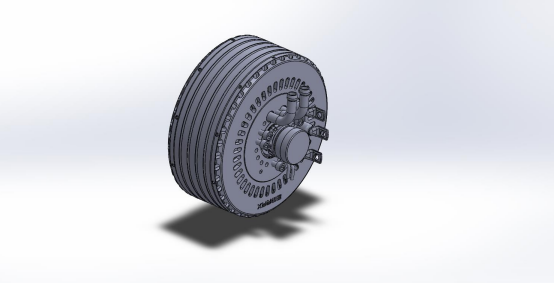
\includegraphics[width=0.6\textwidth]{texfiles/mech/eimg/propulsion/picture_motor}
\caption{CAD of EMRAX 188}
\label{}
\end{figure}

As previously mentioned, we are once again using our EMARX 188 electric motor from last season. You can find all the technical details in Table~\ref{tab: Motor Specifications} .



\subsubsection{Motorshaft}

\begin{figure}[ht!]
  \centering
  \begin{subfigure}{.5\textwidth}
    \centering
    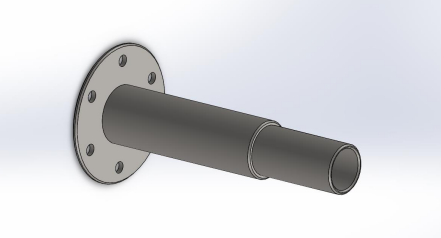
\includegraphics[width=\linewidth]{texfiles/mech/eimg/propulsion/picture_motorshaft}
    \caption{CAD Render}
    \label{fig:CAD Motorshaft}
  \end{subfigure}%
  \begin{subfigure}{.4\textwidth}
    \centering
    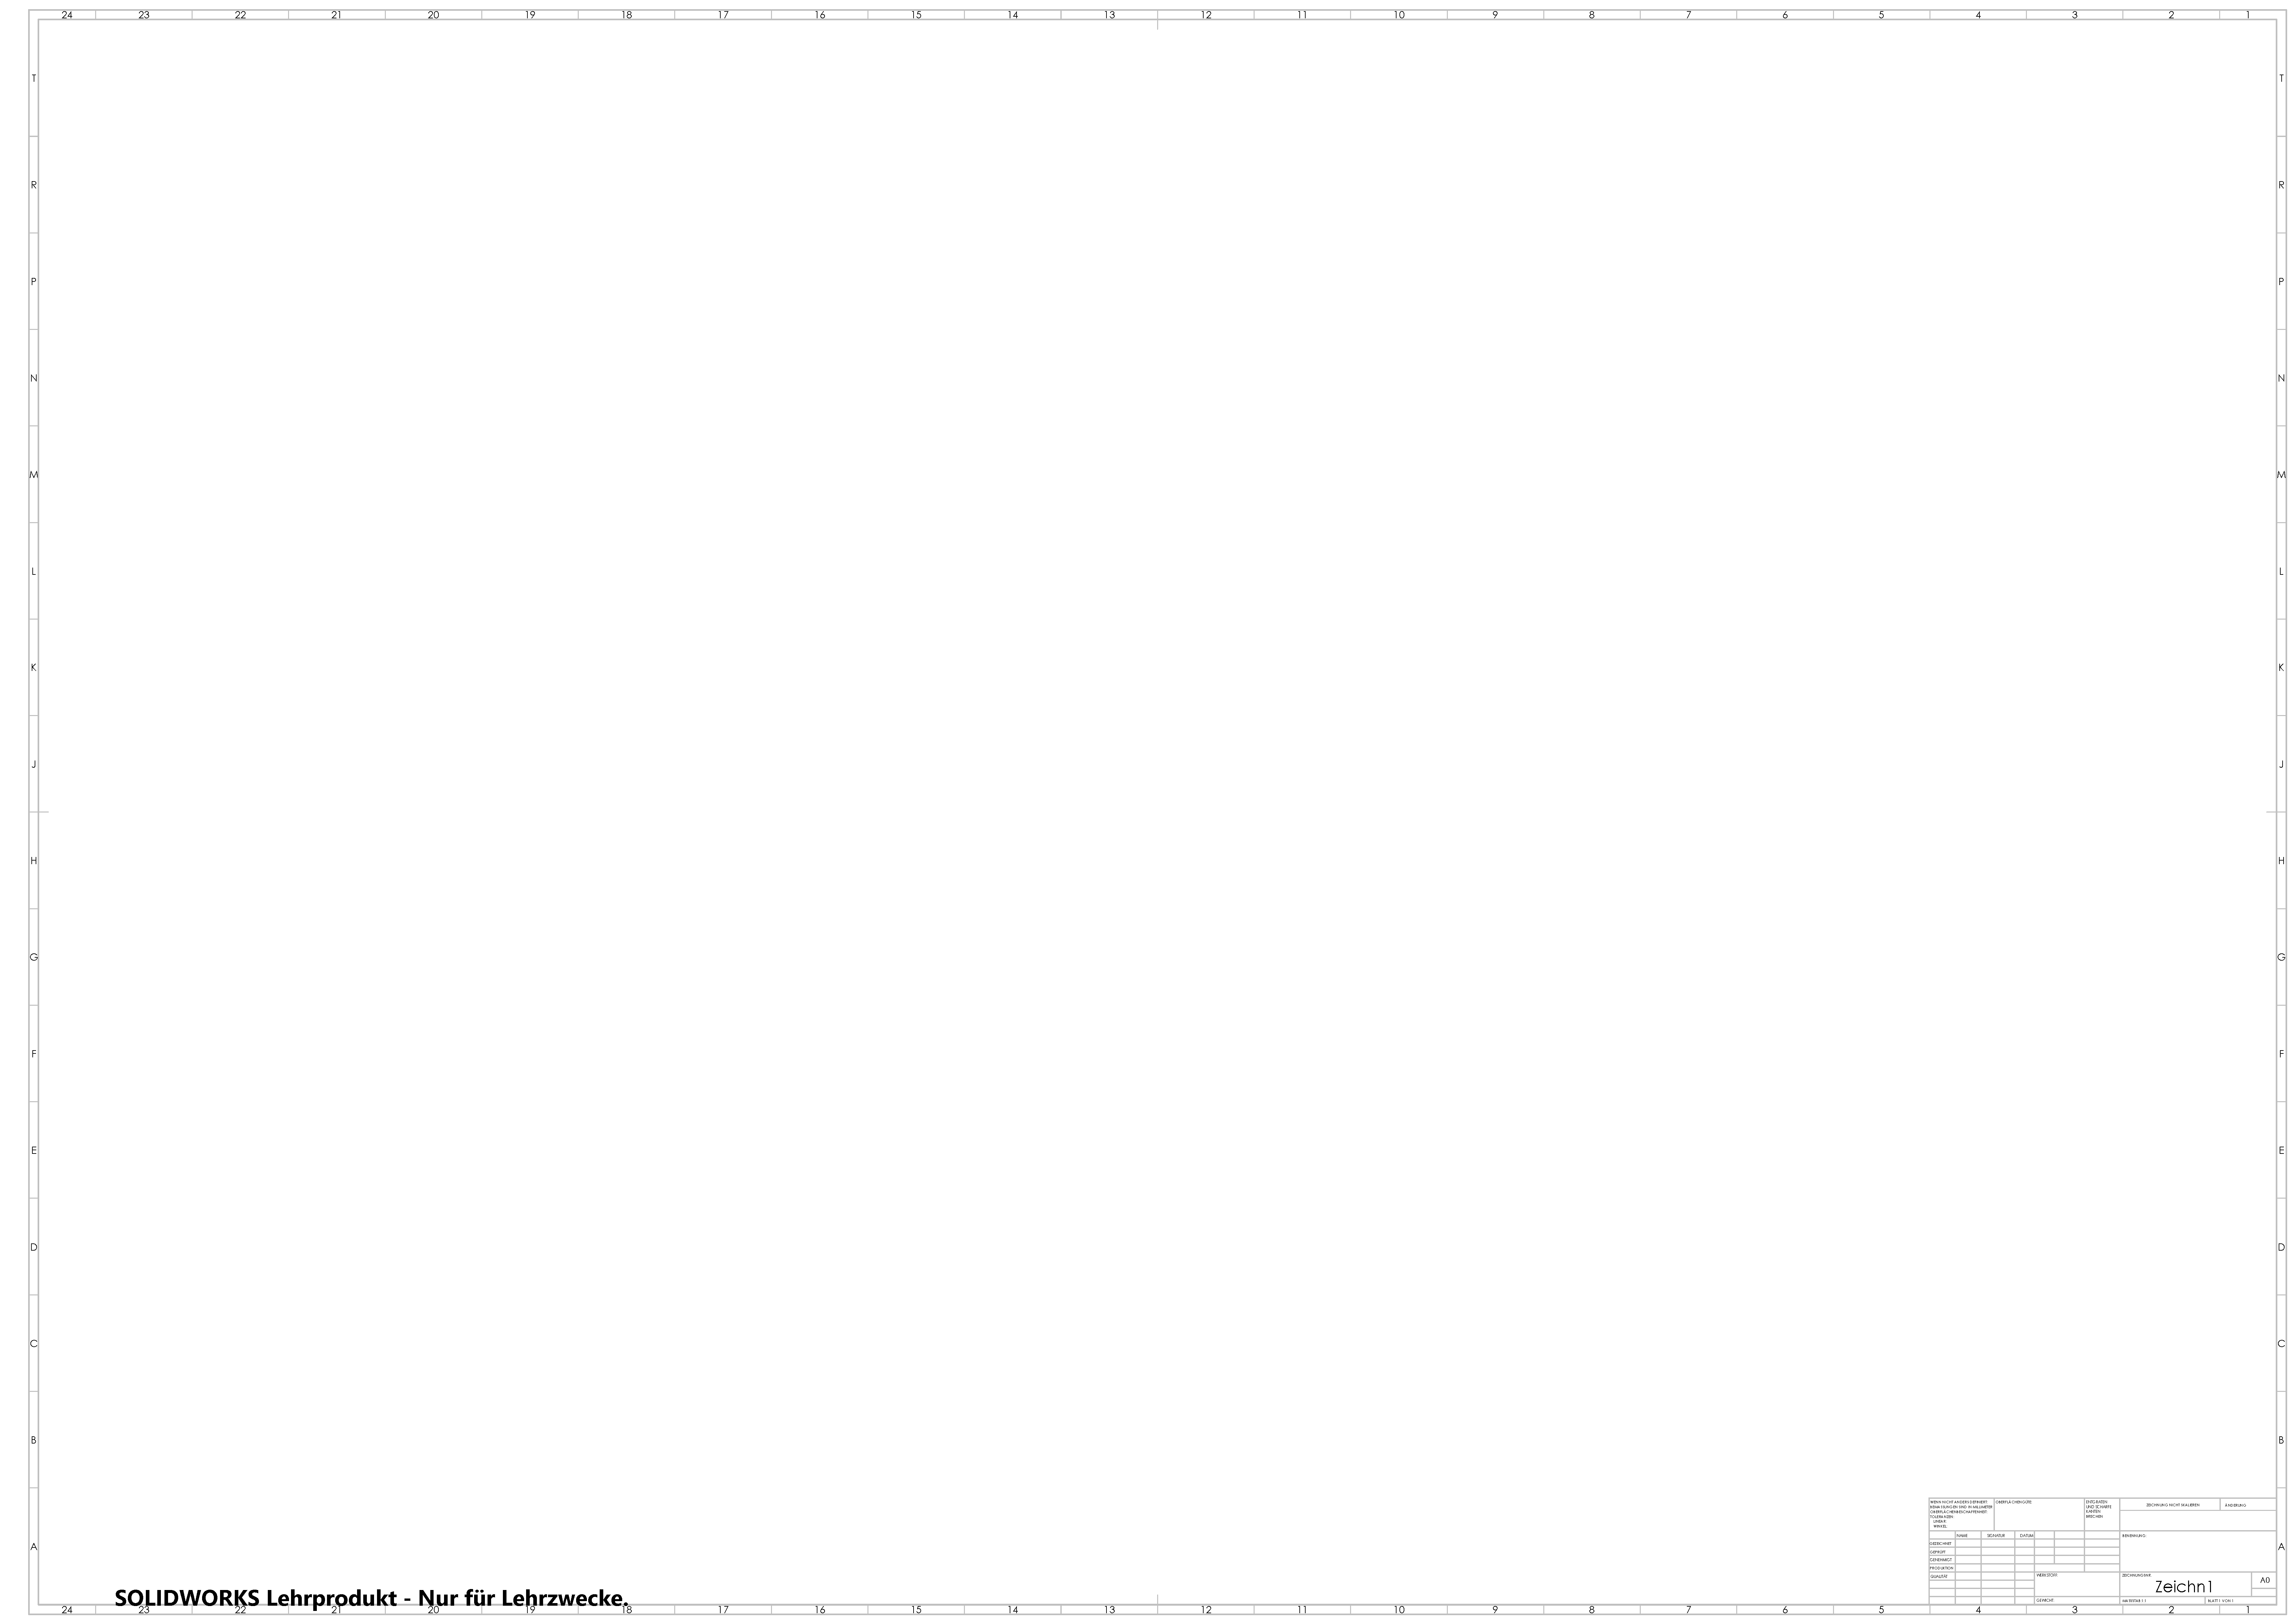
\includegraphics[width=\linewidth]{texfiles/mech/eimg/propulsion/spaceholder_technical_drawing}
    \caption{Technical Drawing}
    \label{fig:TD Motorshaft}
  \end{subfigure}
  \caption{Motor Bracket}
  \label{fig:Motorshaft}
\end{figure}



Even though it is a heavy material, C45 steel provides adequate tensile strength to transmit torque from the motor to the gearbox or from the gearbox to the wheels. To maintain a relatively low weight for this part, it is hollow like all the other shafts. In Figure \ref{fig:motorshaft_forces}, you can now see the applied forces. The shaft is mounted on the motor at the screw holes of the flange (green). This means that the motor torque of \(100 \, \text{Nm}\) (pink) acts up to the surface on which the bevel gear is pressed. The calculation of the contact pressure of \(16.26 \, \text{MPa}\) is given by
\[
p_{\text{contact}}=\frac{2\cdot M\cdot S_r}{\pi \cdot D^2 \cdot l\cdot \mu}
\]
In addition, there is a centrifugal force (blue) at maximum rotational speed of \(6000 \, \text{rpm}\).

\autoref{fig:motorshaft_forces}
\begin{figure}[H]
\centering
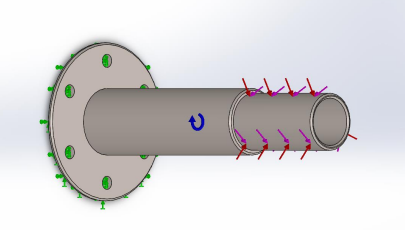
\includegraphics[width=0.6\textwidth]{texfiles/mech/eimg/propulsion/picture_forces_motorshaft}
\caption{Forces acting on the Motorshaft}
\label{fig:motorshaft_forces}
\end{figure}

\subsubsection{Bevel Gears}
picture gearbox

The bevel gears with the article numbers 36736000 and 36736100 are our choice to fulfill the desired purpose.
36736000 offers spur gearing with 20 teeth. With a maximum permissible torque of 130 Nm, it can withstand the prevailing forces. 
The larger counterpart 36736100 therefore has twice as many teeth (40 teeth) and is designed for a maximum torque of 260 Nm.

\subsubsection{Gearshafts}
\begin{figure}[H]
\centering
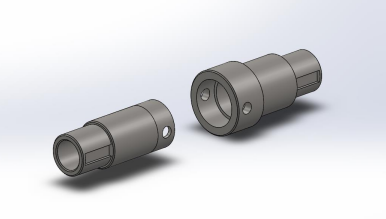
\includegraphics[width=0.6\textwidth]{texfiles/mech/eimg/propulsion/picture_gearshafts}
\caption{}
\label{}
\end{figure}

To be able to conduct the torque of the bevel gear, we have designed another shaft. This consists of two individual parts, one which is again pressed into the bevel gear and the other which is screwed onto the first part after pressing.
The specifications of the initially acting shaft are as follows:

\begin{figure}[ht!]
  \centering
  \begin{subfigure}{.5\textwidth}
    \centering
    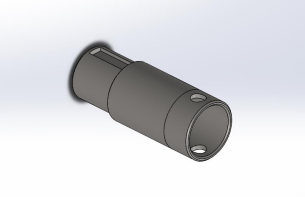
\includegraphics[width=\linewidth]{texfiles/mech/eimg/propulsion/picture_gearshaft_right}
    \caption{CAD Render}
    \label{fig:CAD Motorshaft}
  \end{subfigure}%
  \begin{subfigure}{.5\textwidth}
    \centering
    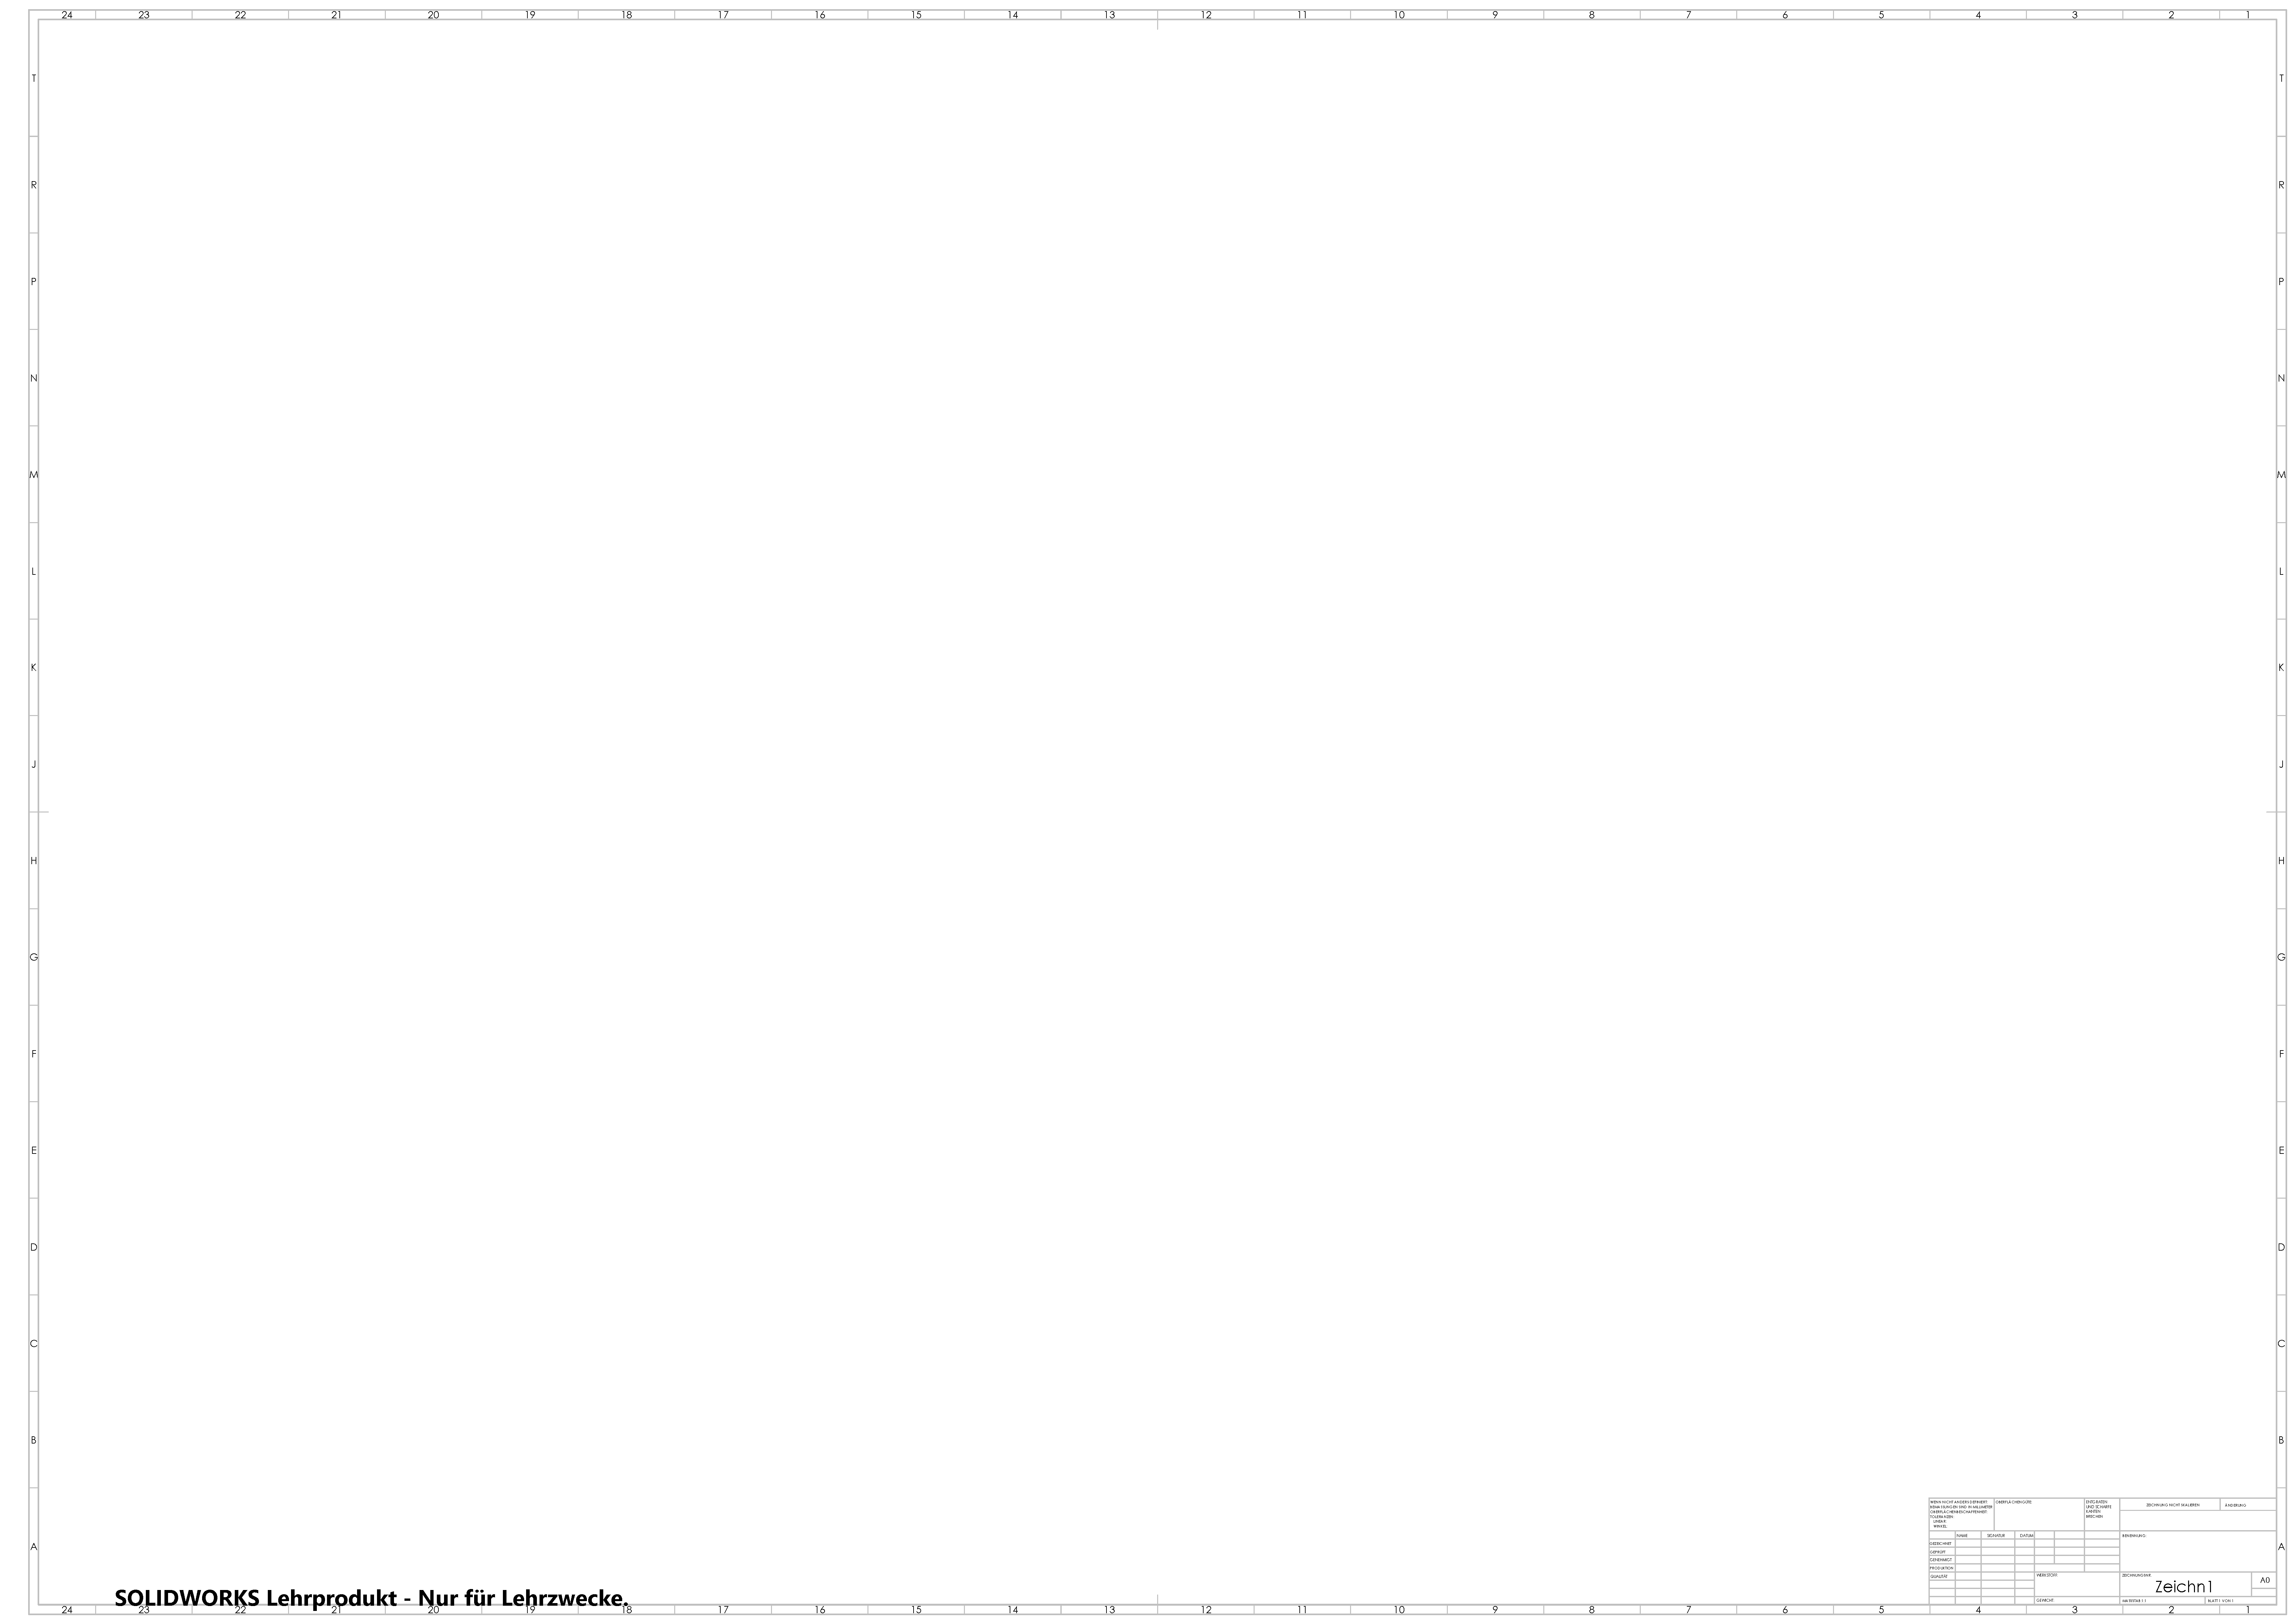
\includegraphics[width=\linewidth]{texfiles/mech/eimg/propulsion/spaceholder_technical_drawing}
    \caption{Technical Drawing}
    \label{fig:TD Motorshaft}
  \end{subfigure}
  \caption{Motor Bracket}
  \label{fig:Motorshaft}
  \end{figure}



Fig.xx  shows all the acting forces. For calculating the pressing force (red) we again use the formula for \(p_{\text{contact}}\)
and get the result of \(21.22 \, \text{MPa}\). The higher torque of \(200 \, \text{Nm}\) (pink) resulting from the gear ratio also acts on this surface and is transferred to the screw holes and keyway (green). A centrifugal force (blue) also acts on this part, but this has now been halved by the gear ratio and is therefore only based on \(3000 \, \text{rpm}\). Finally, we assume a bearing restraint (orange) at the shaft end to the shaft joint. The admissibility of this case is described in the paragraph on the shaft joint itself.

\begin{figure}[H]
\centering
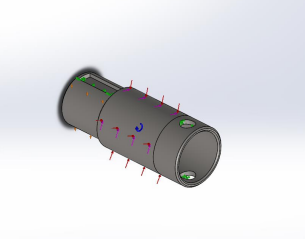
\includegraphics[width=0.6\textwidth]{texfiles/mech/eimg/propulsion/picture_forces_gearshaft_right}
\caption{Forces acting on the pressfitted Gearshaft}
\label{fig:gearshaft_right_forces}
\end{figure}


The torque is now transferred to the second part of the gearshaft:
\begin{figure}[ht!]
  \centering
  \begin{subfigure}{.5\textwidth}
    \centering
    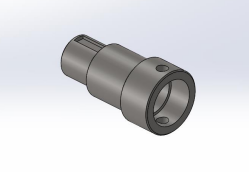
\includegraphics[width=\linewidth]{texfiles/mech/eimg/propulsion/picture_gearshaft_left}
    \caption{CAD Render}
    \label{fig:CAD Motorshaft}
  \end{subfigure}%
  \begin{subfigure}{.5\textwidth}
    \centering
    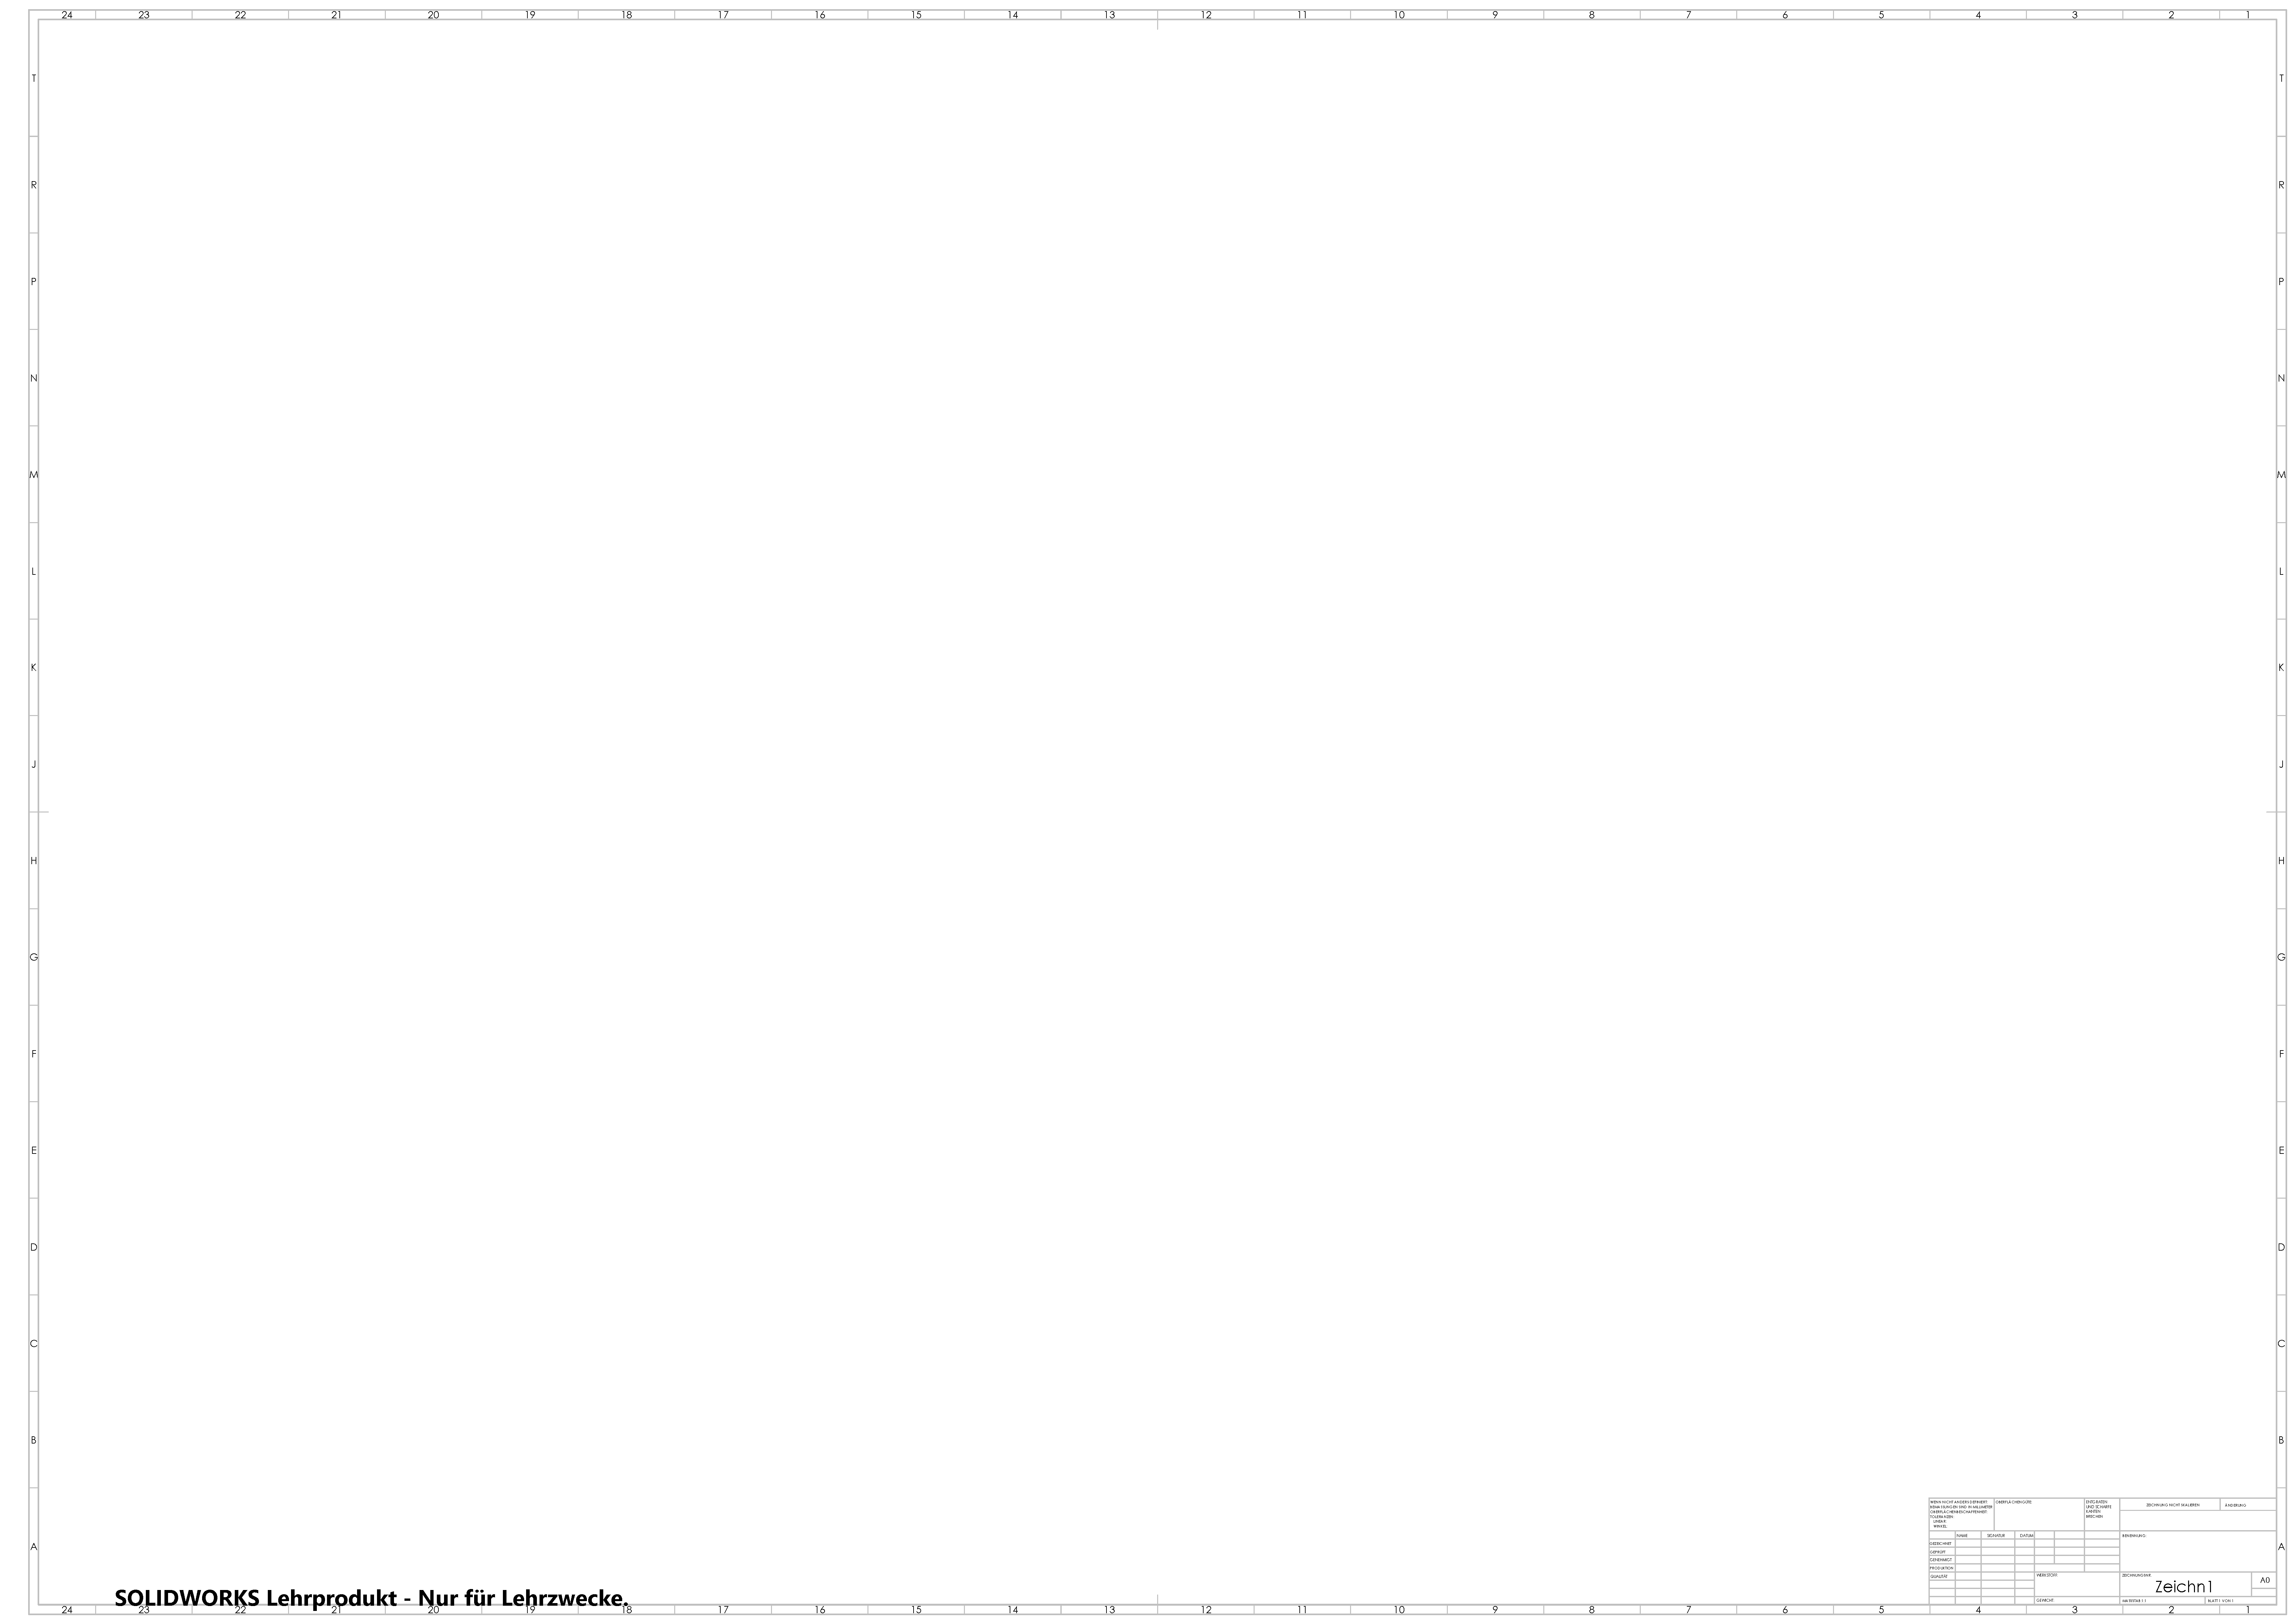
\includegraphics[width=\linewidth]{texfiles/mech/eimg/propulsion/spaceholder_technical_drawing}
    \caption{Technical Drawing}
    \label{fig:TD Motorshaft}
  \end{subfigure}
  \caption{Motor Bracket}
  \label{fig:Motorshaft}
  \end{figure}



Fig.xx shows all the forces acting on this part. The two shafts are connected to each other at the screw holes (green). The centrifugal force (blue) acts as in the first shaft at \(3000 \, \text{rpm}\) and the torque of \(200 \, \text{Nm}\) (pink) up to the keyway. This end piece of the shaft is also simulated as a bearing (orange).

\begin{figure}[H]
\centering
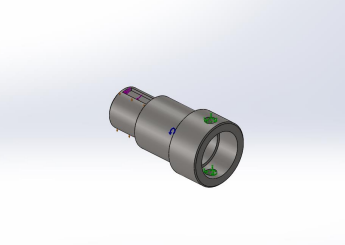
\includegraphics[width=0.6\textwidth]{texfiles/mech/eimg/propulsion/picture_forces_gearshaft_left}
\caption{Forces acting on the bolted Gearshaft}
\label{fig:gearshaft_left_forces}
\end{figure}

\subsubsection{Shaft Joints}
\begin{figure}[H]
\centering
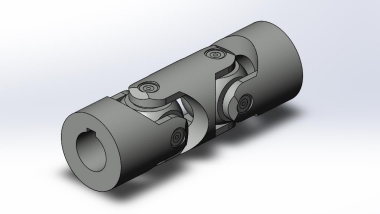
\includegraphics[width=0.6\textwidth]{texfiles/mech/eimg/propulsion/picture_shaft_joint}
\caption{}
\label{}
\end{figure}


To enable the system to absorb shocks, we use cardan shafts on each side. This allows the wheels to move vertically independently of the rest of the pod. Our partner Mädler is once again supplying us with such complex parts. Item number 63167000N is a double universal joint which we install in our system. It has a keyway at both ends and is designed to transmit 202 Nm at 3000 rpm. These specifications are almost perfect for our drive power.
We will mount the heart of our system at the ends of this joint adjacent to the gearbox. This is also the reason why a bearing is created at the respective ends in the simulations of the shafts because this bearing is also attached above the respective area.
However, more on the bearing and attachment points will follow in the corresponding sections.

\subsubsection{Wheelshafts}
\begin{figure}[ht!]
  \centering
  \begin{subfigure}{.5\textwidth}
    \centering
    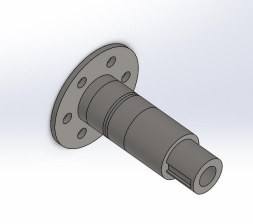
\includegraphics[width=\linewidth]{texfiles/mech/eimg/propulsion/picture_wheelshaft}
    \caption{CAD Render}
    \label{fig:CAD Motorshaft}
  \end{subfigure}%
  \begin{subfigure}{.5\textwidth}
    \centering
    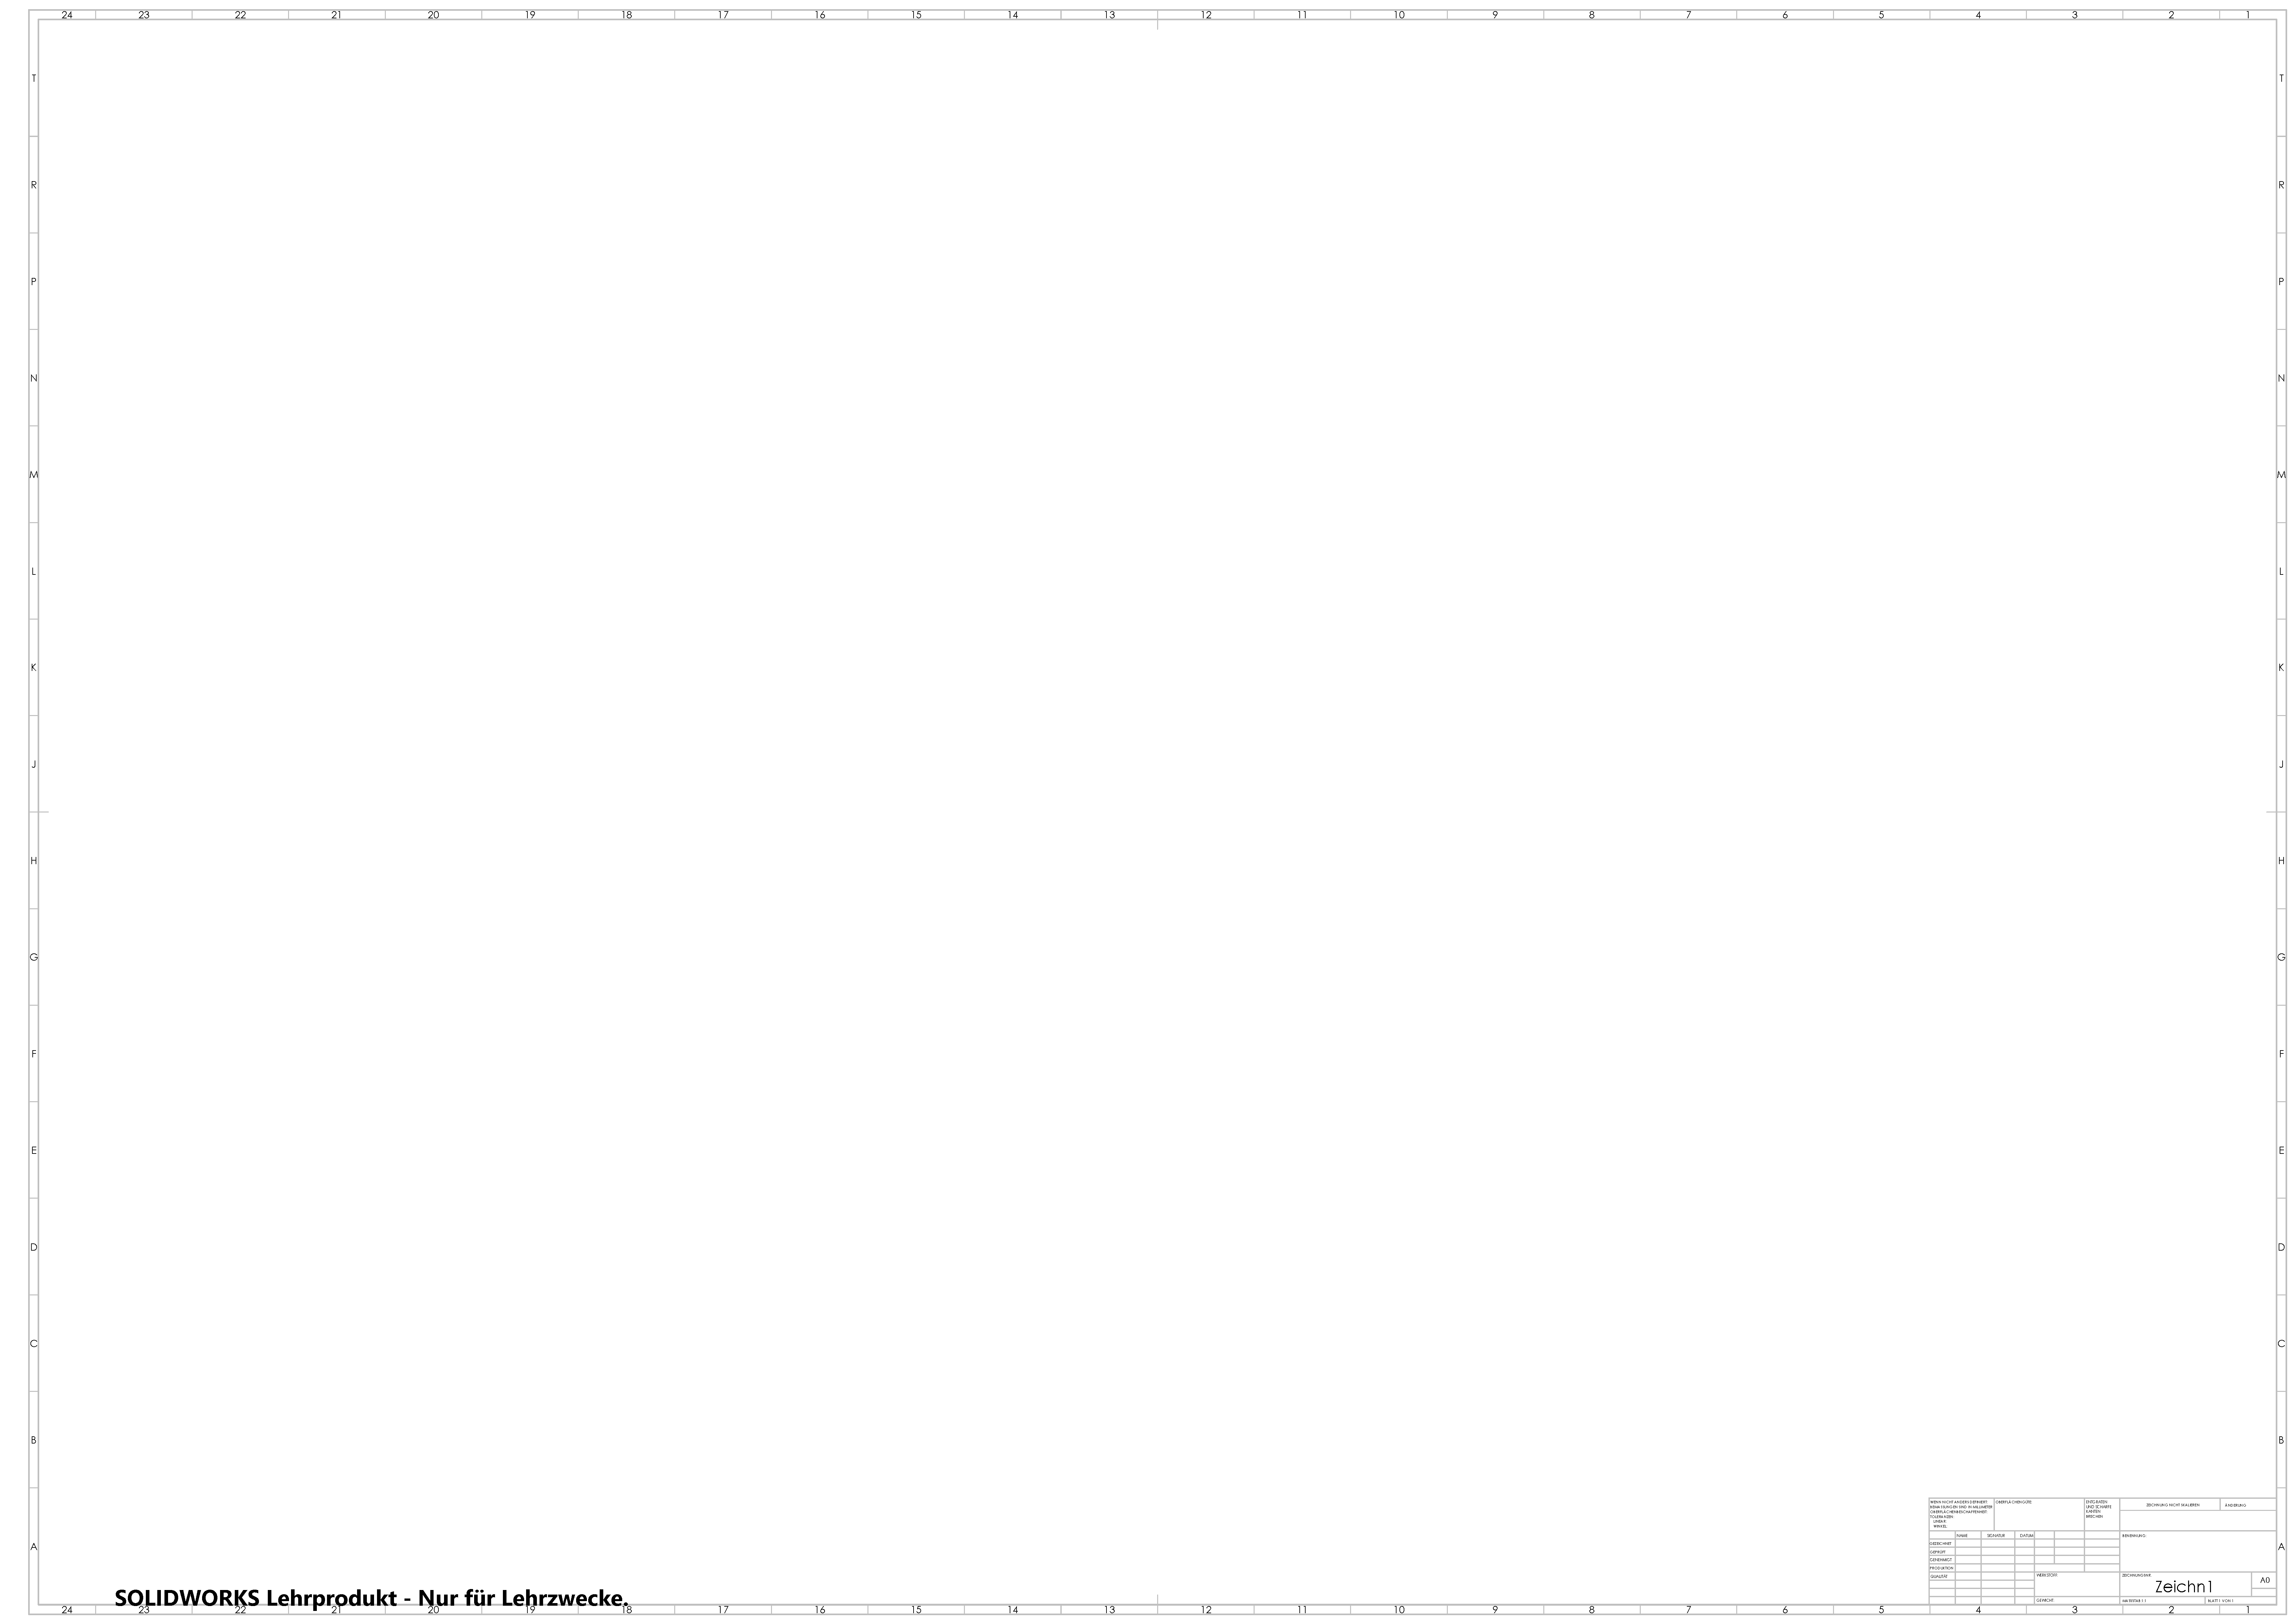
\includegraphics[width=\linewidth]{texfiles/mech/eimg/propulsion/spaceholder_technical_drawing}
    \caption{Technical Drawing}
    \label{fig:TD Motorshaft}
  \end{subfigure}
  \caption{Motor Bracket}
  \label{fig:Motorshaft}
  \end{figure}


The wheel shafts provide the mounting point for the wheels. This is done by means of a bolt circle on a flange to ensure easy mounting and, if necessary, changing of the wheels. In this shaft, the 200 Nm torque (pink) applied to the keyway is transmitted to the wheel over the entire surface of the flange. The centrifugal force (blue) is also generated again due to the 3000 rpm and this shaft is also mounted on bearings (orange) within the knuckles. You can find out more about this bearing in the suspension section. However, this shaft must be able to withstand the mass inertia of the wheel (red). This is calculated by
\(5/2 \times m_{\text{wheel}} \times a\)

\begin{figure}[ht]
\centering
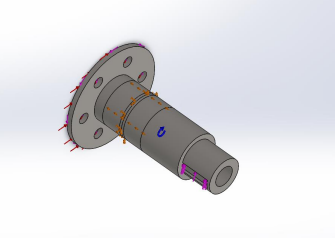
\includegraphics[width=0.6\textwidth]{texfiles/mech/eimg/propulsion/picture_forces_wheelshaft}
\caption{Forces acting on the wheelshaft}
\label{fig:wheelshaft_forces}
\end{figure}

\subsubsection{Wheels}
\begin{figure}[ht!]
  \centering
  \begin{subfigure}{.5\textwidth}
    \centering
    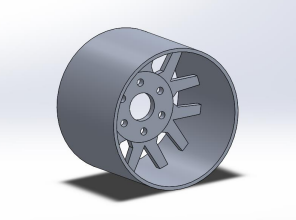
\includegraphics[width=\linewidth]{texfiles/mech/eimg/propulsion/picture_wheel}
    \caption{CAD Render}
    \label{fig:CAD Motorshaft}
  \end{subfigure}%
  \begin{subfigure}{.5\textwidth}
    \centering
    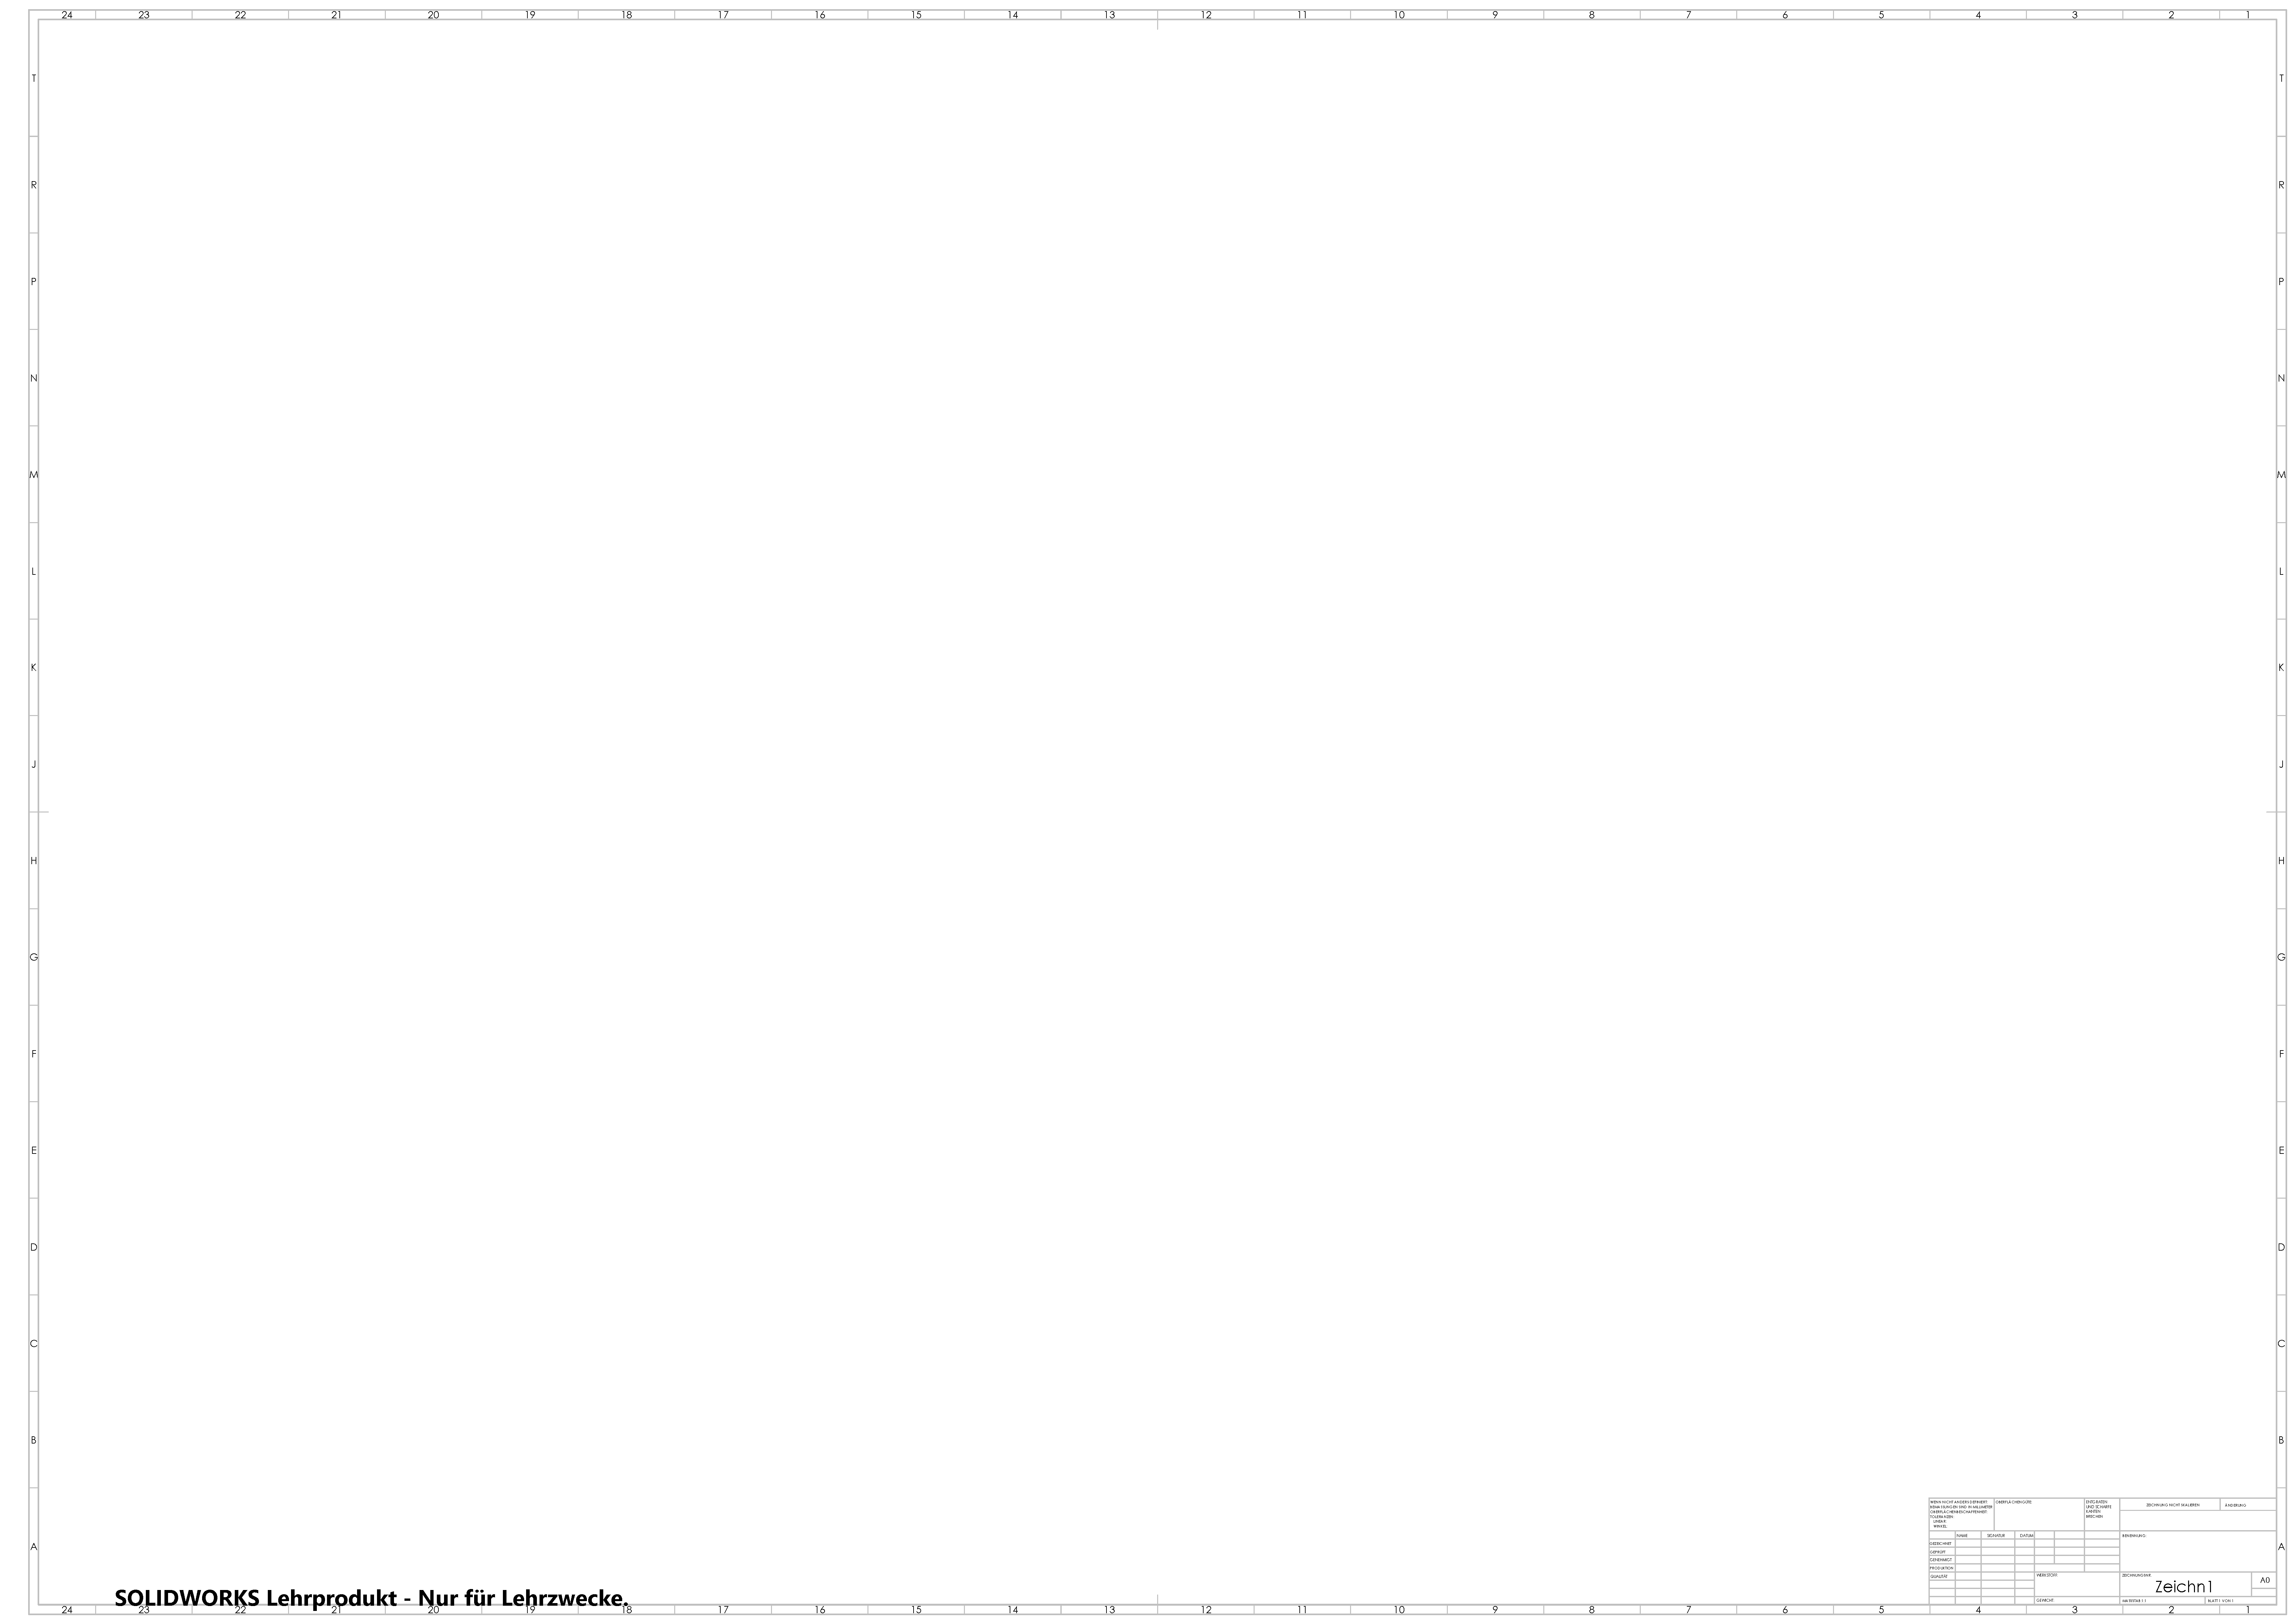
\includegraphics[width=\linewidth]{texfiles/mech/eimg/propulsion/spaceholder_technical_drawing}
    \caption{Technical Drawing}
    \label{fig:TD Motorshaft}
  \end{subfigure}
  \caption{Motor Bracket}
  \label{fig:Motorshaft}
 
\end{figure}

Finally, we transfer the torque (pink) to the wheels via the contact surface of the flange (green). The mass inertia of the wheel (red)
\(5/2 \times m_{\text{wheel}} \times a\)
, again the centrifugal force at 3000 rpm (blue) and the local pod weight of approximately 600 N (orange) also have an effect here. This weight, together with the rolling friction coefficient of the rubber cover, enables slip-free propulsion. We get this coefficient of 0,5099 by the formula
\[
\frac{m \cdot a}{m \cdot g}
\]

\begin{figure}[H]
\centering
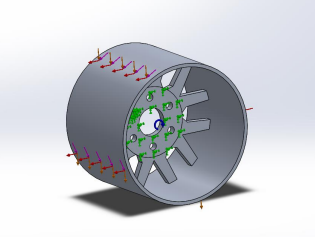
\includegraphics[width=0.6\textwidth]{texfiles/mech/eimg/propulsion/picture_forces_wheel}
\caption{Forces acting on the wheels}
\label{fig:wheel_forces}
\end{figure}


\subsubsection{Motorbracket}

\begin{figure}[ht!]
  \centering
  \begin{subfigure}{.5\textwidth}
    \centering
    \includegraphics[width=\linewidth]{texfiles/mech/eimg/propulsion/placeholder}
    \caption{CAD Render}
    \label{fig:CAD Motorbracket}
  \end{subfigure}%
  \begin{subfigure}{.5\textwidth}
    \centering
    \includegraphics[width=\linewidth]{texfiles/mech/eimg/propulsion/placeholder}
    \caption{Technical Drawing}
    \label{fig:TD Motorbracket}
  \end{subfigure}
  \caption{Motor Bracket}
  \label{fig:Motorbracket}
\end{figure}

Our motor is mounted in the chassis using a bracket. This contains all the holes for screws and other components that protrude to the rear. End plates with screw holes are welded to four arms to finally screw () them into the chassis. The torque () and the inertia of the motor () prevail at this bracket.

\begin{figure}[H]
\centering
\includegraphics[width=0.6\textwidth]{texfiles/mech/eimg/propulsion/placeholder}
\caption{Forces acting on the motorbracket}
\label{fig:motorbracket_forces}
\end{figure}

\subsubsection{Motorshaftbracket}
\begin{figure}[H]
\centering
\includegraphics[width=0.6\textwidth]{texfiles/mech/eimg/propulsion/placeholder}
\caption{}
\label{}
\end{figure}

\begin{figure}[H]
\centering
\includegraphics[width=0.6\textwidth]{texfiles/mech/eimg/propulsion/placeholder}
\caption{}
\label{}
\end{figure}

To finally support this first area of the drive system, we also support the shaft that protrudes from the motor. This is done using the CHDF35 flangebearing from Misumi. This bearing is finally integrated into the chassis by another bracket. Only the weight of the motor shaft (), its mass inertia and the wheight of the flangebearing () act on this bracket.

%\begin{figure}[H]
%\centering
%\includegraphics[width=0.6\textwidth]{texfiles/mech/eimg/propulsion/picture_forces_motorshaftbracket}
%\caption{Forces acting on the motorshaftbracket}
%\label{fig:motorshaftbracket_forces}
%\end{figure}

\subsubsection{Bearinghouse}
%\begin{figure}[H]
%\centering
%\includegraphics[width=0.6\textwidth]{texfiles/mech/eimg/propulsion/picture_bearinghouse}
%\caption{}
%\label{}
%\end{figure}

%\begin{figure}[H]
%\centering
%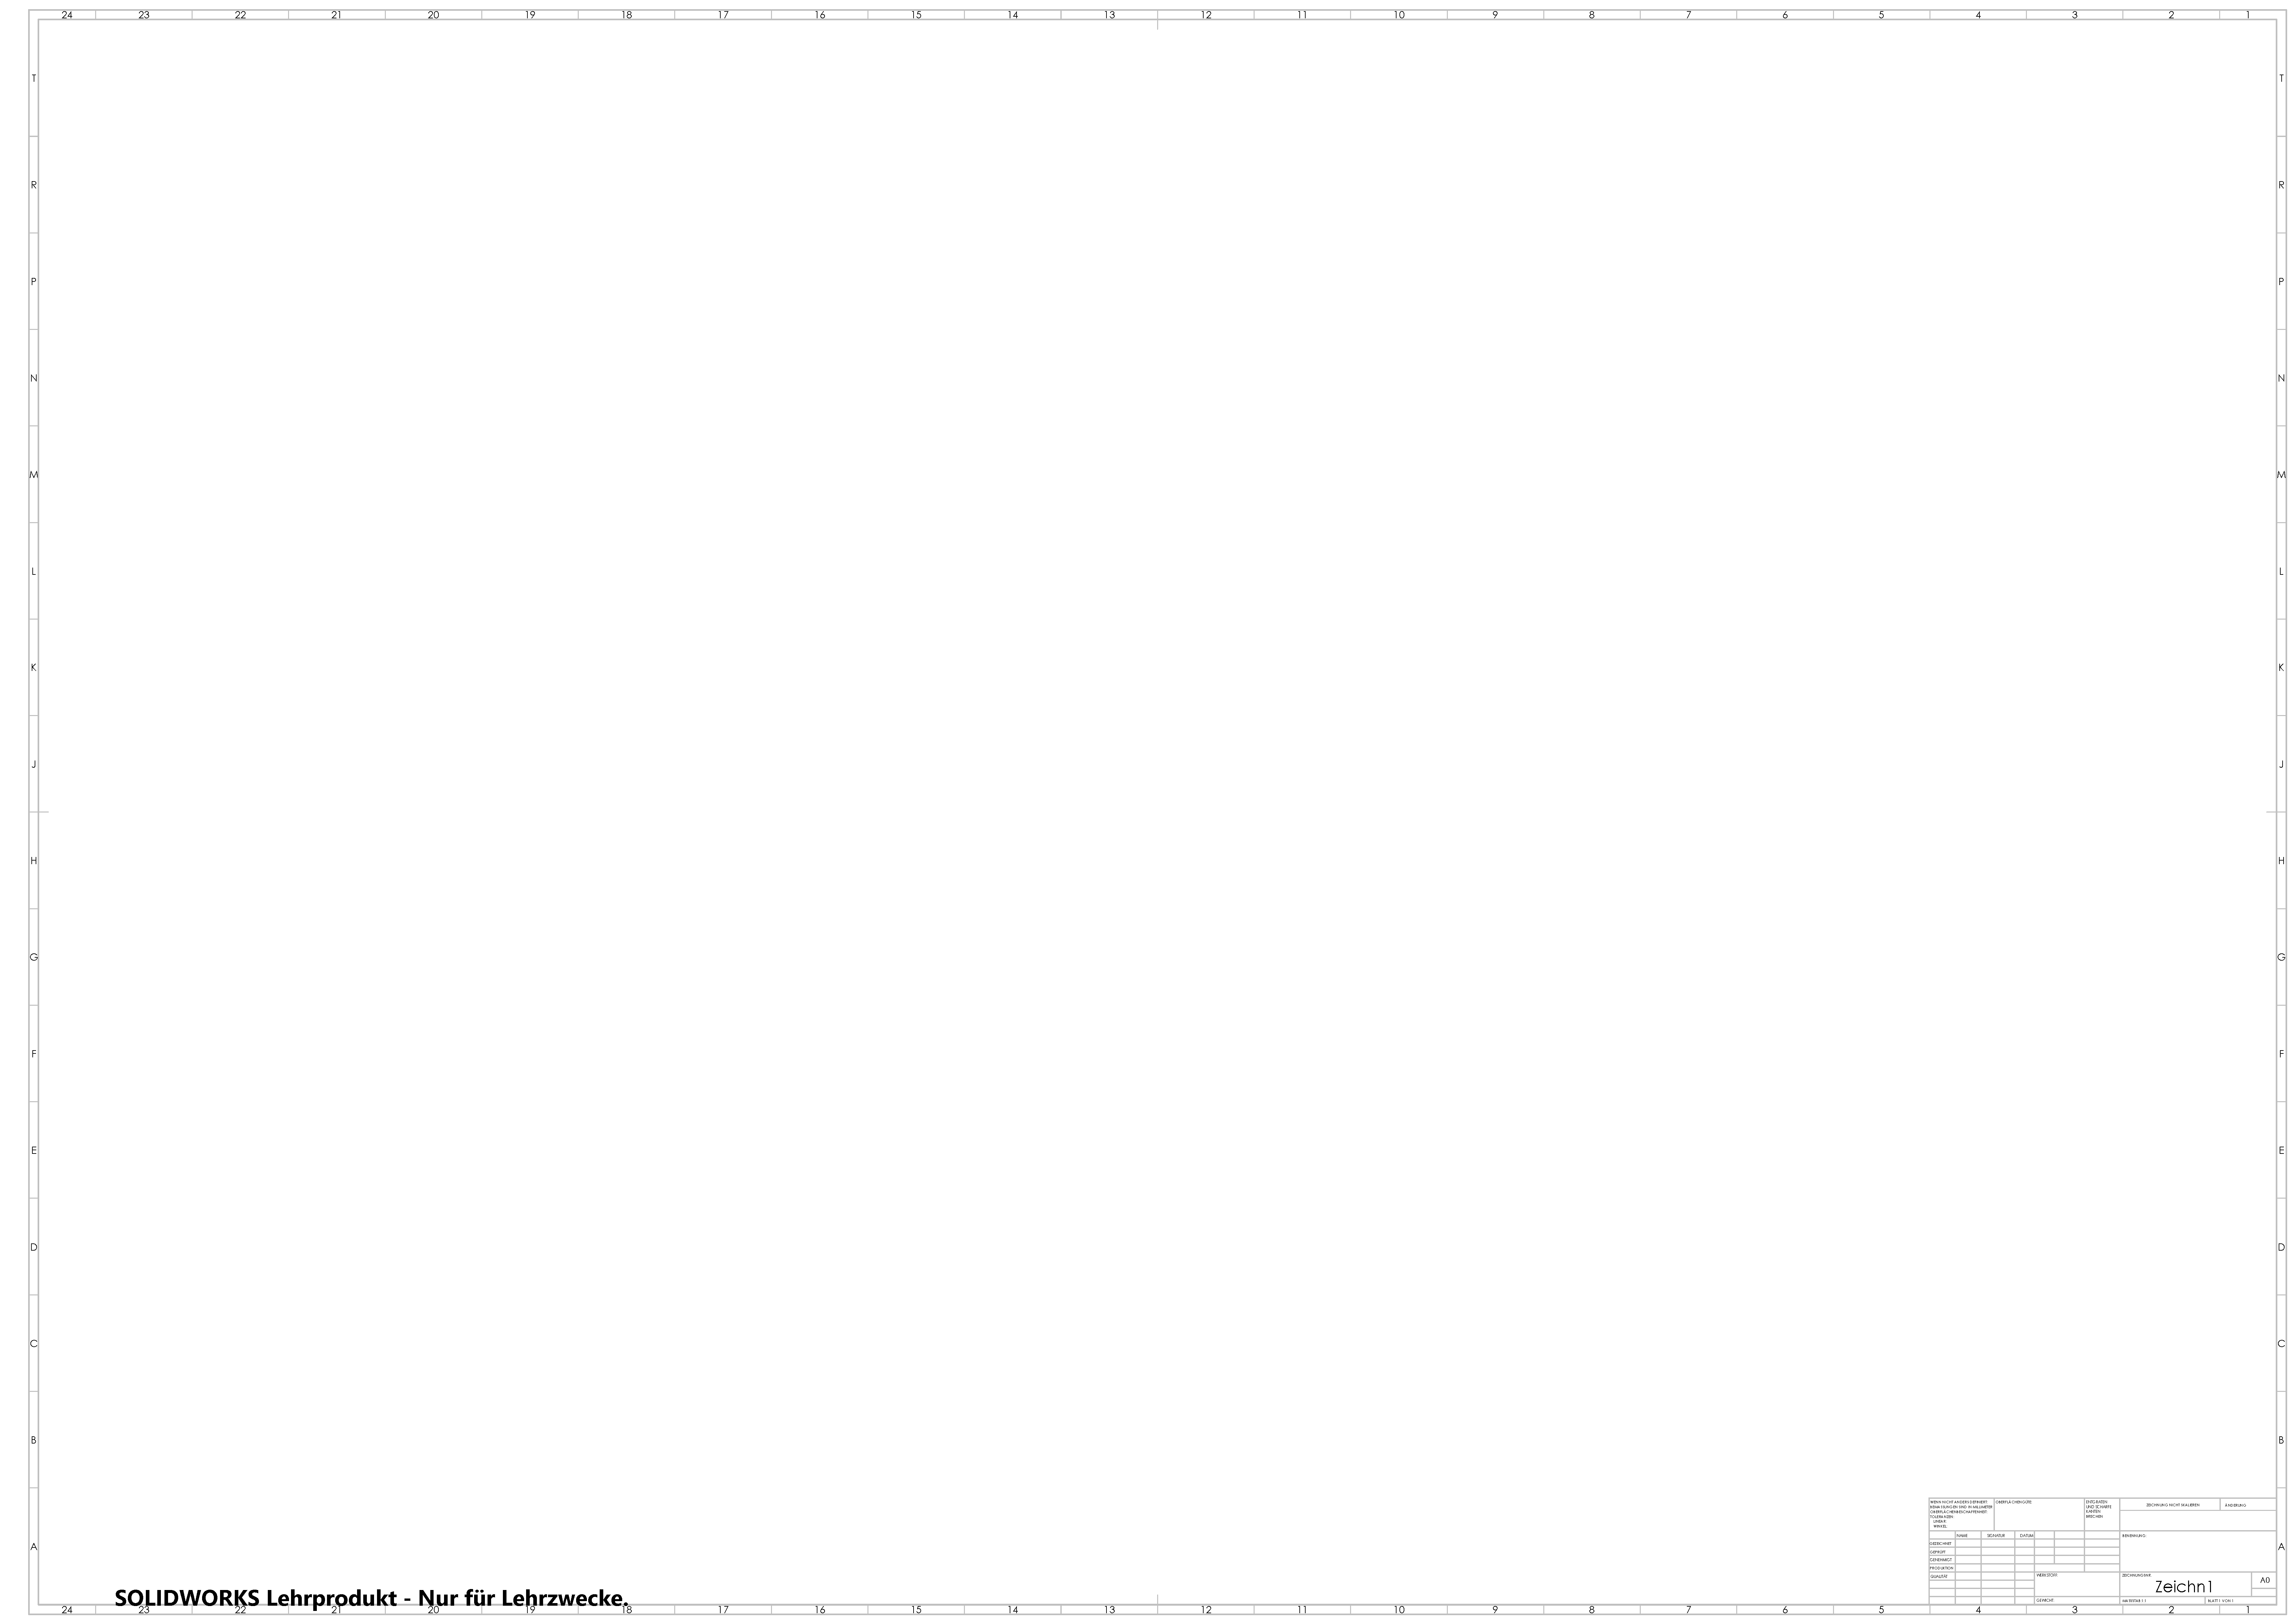
\includegraphics[width=0.6\textwidth]{texfiles/mech/eimg/propulsion/spaceholder_technical_drawing}
%\caption{}
%\label{}
%\end{figure}

To provide sufficient support for the drive axle, we mount it at two points. For space reasons, we designed the bearinghouse ourselves. The weight of the axle (pink) acts on this bearinghouse at the respective point, as well as its mass moment of inertia (). This bearing shell is installed with screws (green) on another bracket in the chassis.

%\begin{figure}[H]
%\centering
%\includegraphics[width=0.6\textwidth]{texfiles/mech/eimg/propulsion/picture_forces_bearinghouse}
%\caption{Forces acting on the bearinghouses}
%\label{fig:bearinghouse_forces}
%\end{figure}


\subsubsection{Bearingbracket}
%\begin{figure}[H]
%\centering
%\includegraphics[width=0.6\textwidth]{texfiles/mech/eimg/propulsion/picture_bearingbracket}
%\caption{}
%\label{}
%\end{figure}

%\begin{figure}[H]
%\centering
%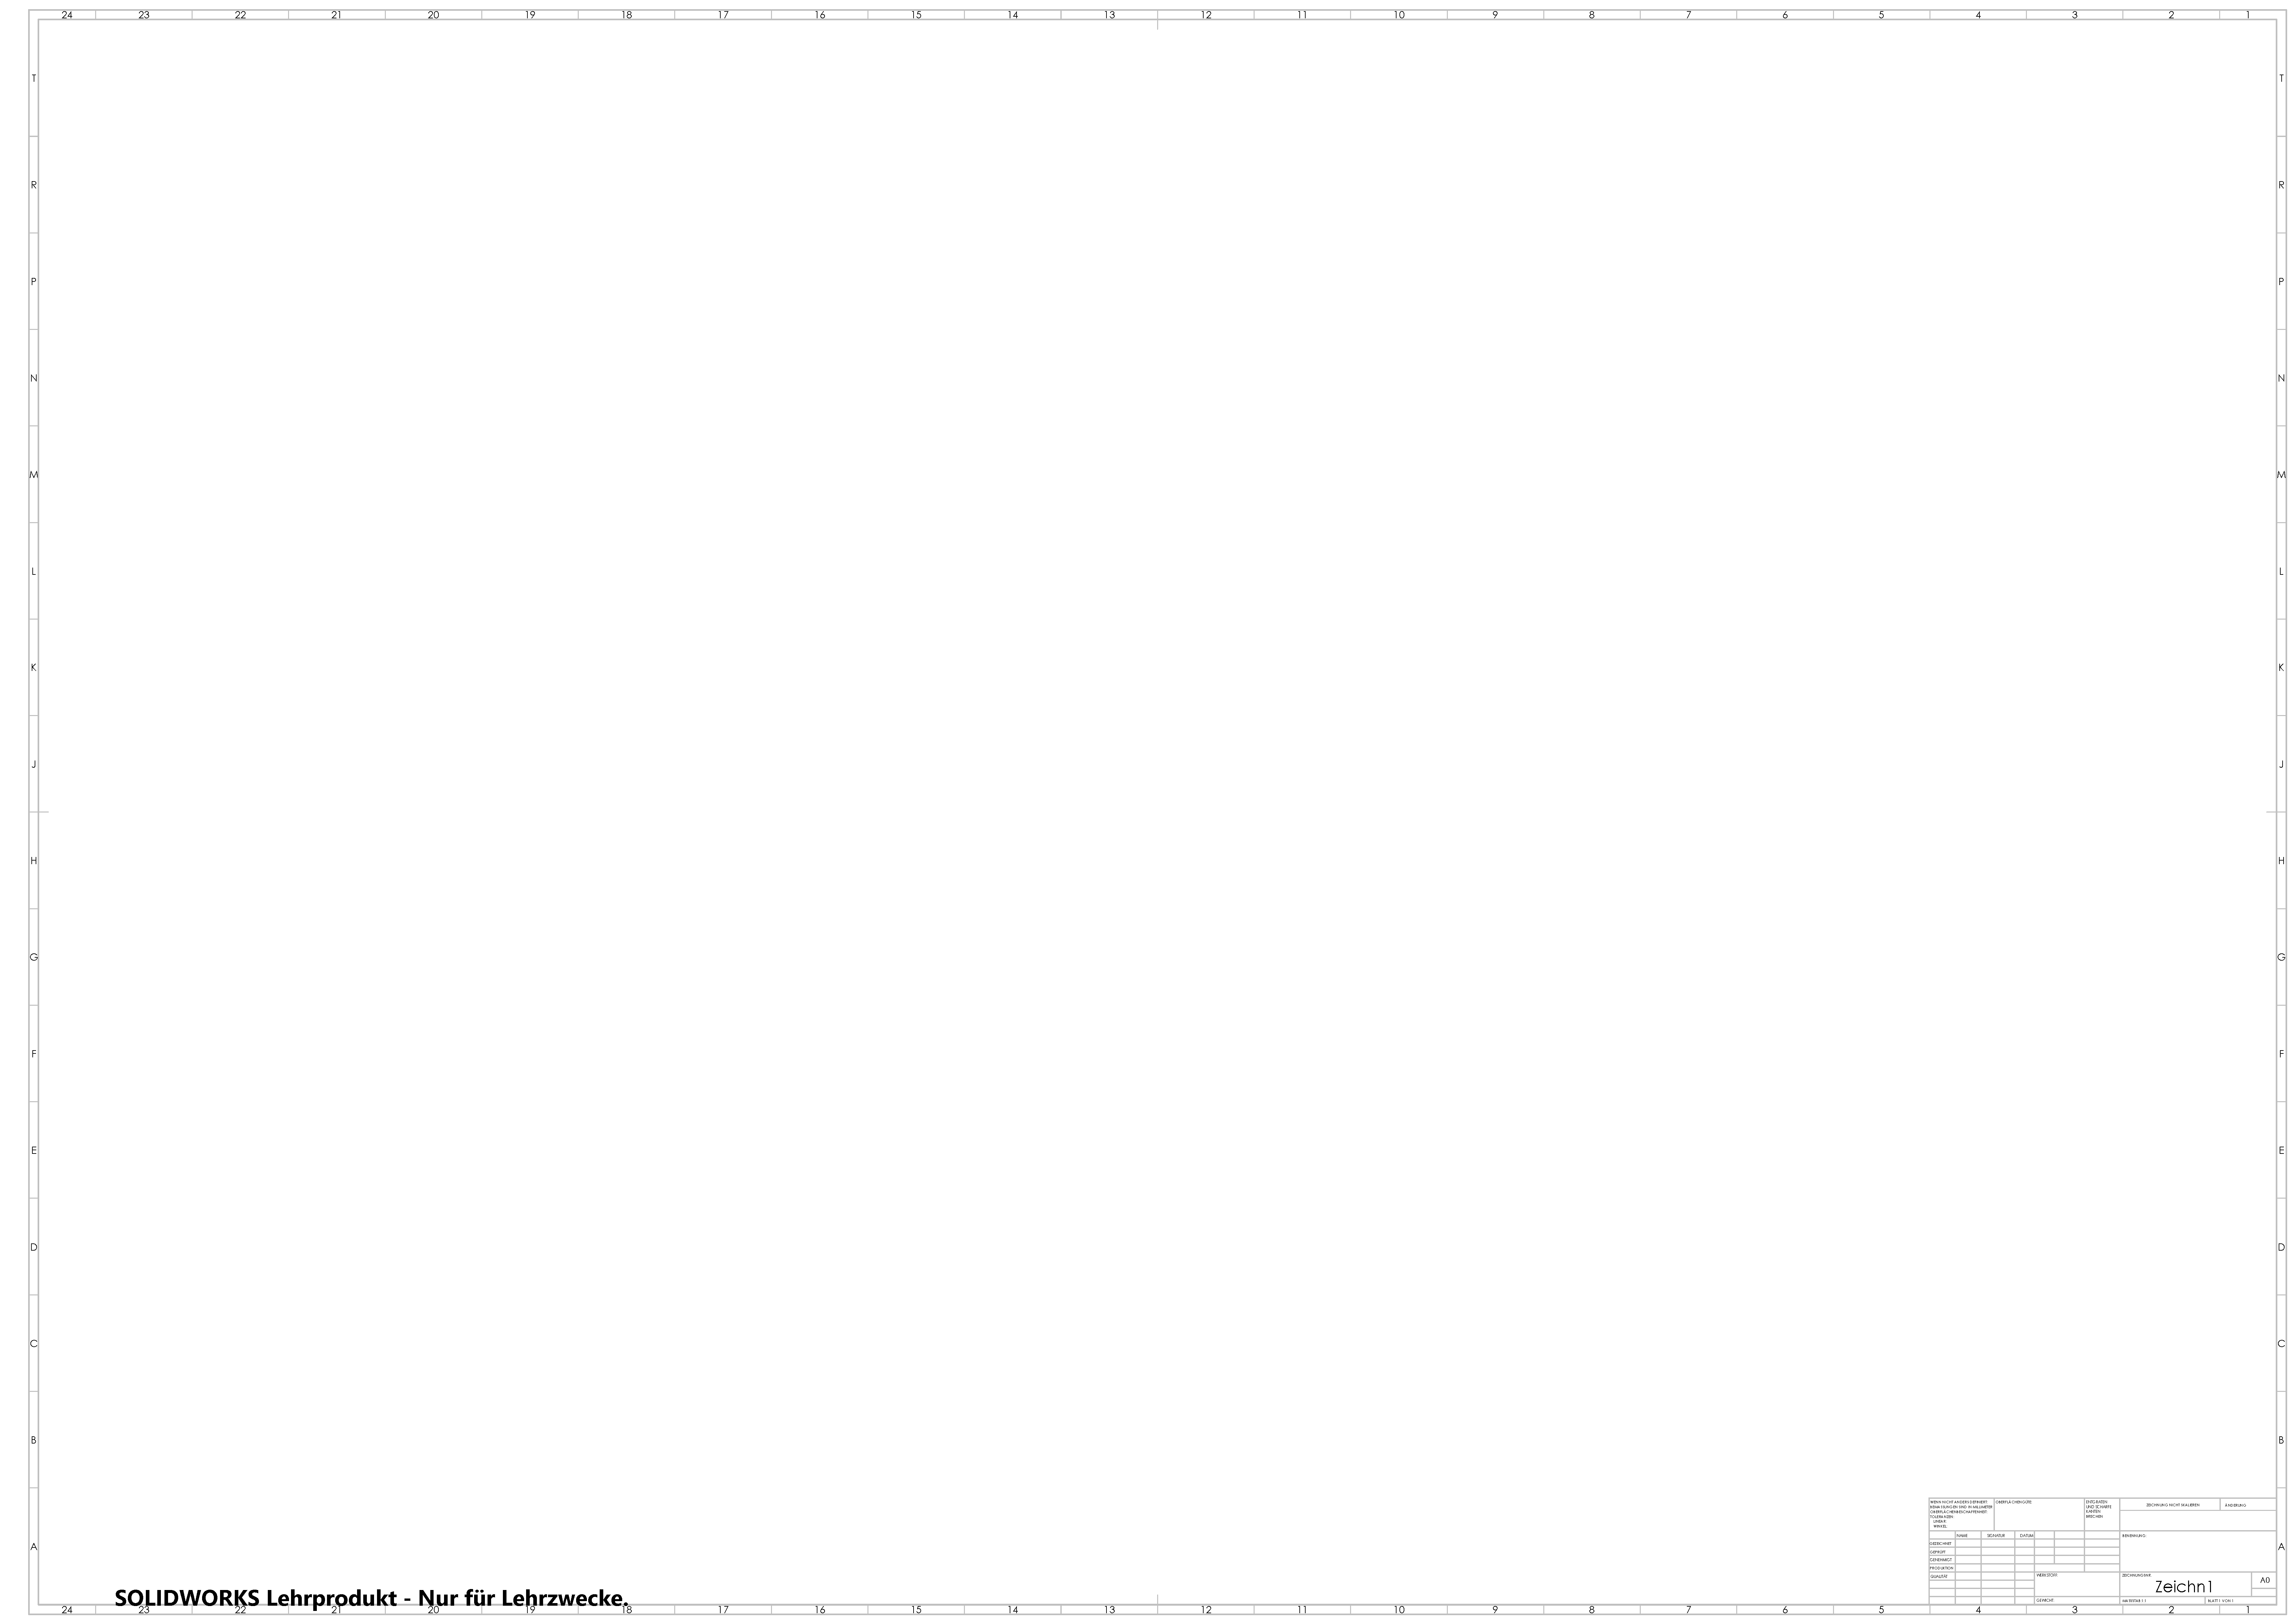
\includegraphics[width=0.6\textwidth]{texfiles/mech/eimg/propulsion/spaceholder_technical_drawing}
%\caption{}
%\label{}
%\end{figure}

As already mentioned, the bearinghouses are mounted on additional brackets. Like the motor brackets, these brackets consist of a plate with screw holes () to which end plates are welded via which the component is installed in the chassis (). The same forces act on this bracket as on the bearinghouse with the weight of the bearinghouse itself ().

%\begin{figure}[H]
%\centering
%\includegraphics[width=0.6\textwidth]{texfiles/mech/eimg/propulsion/picture_forces_bearingbracket}
%\caption{Forces acting on the bearingbrackets}
%\label{fig:bearingbracket_forces}
%\end{figure}

\subsubsection{Materials}
\begin{table}[H]
\centering
\begin{adjustbox}{width=\textwidth}
\begin{tabular}{|>{\bfseries}m{3cm}|m{2cm}|m{2.3cm}|m{2.3cm}|m{2.5cm}|}
\hline
Component & Number & Mass [kg] & Total Mass [kg] & Material \\
\hline
Motor & x1 & 7 & 14 & \\
\hline
Motorshaft & x1 & 0.4 & 0.4 & C45 Steel \\
\hline
Bevelgear z=20 & x1 & 3 & 3 & C45 Steel \\
\hline
Bevelgear z=40 & x1 & 9.6 & 9.6 & C45 Steel \\
\hline
Gearshaft Pressfitted & x1 & 0.3 & 0.3 & C45 Steel \\
\hline
Gearshaft bolted & x1 & 0.7 & 0.7 & C45 Steel \\
\hline
Shaft Joint & x2 & 4.1 & 8.2 & C45 Steel \\
\hline
Wheelshaft & x2 & 0.7 & 1.4 & C45 Steel \\
\hline
Wheel & x2 & 1.7 & 3.4 & Aluminum 6061 \\
\hline
Motorbracket & x1 &  &  & Aluminum 6061 \\
\hline
Motorshaft- bracket and flangebearing & x1 &  &  & Aluminum 6061 \\
\hline
Bearinghouse & x2 &  &  & Aluminum 6061 \\
\hline
Bearingbracket & x2 &  &  & Aluminum 6061 \\
\hline
\end{tabular}
\end{adjustbox}
\caption{Mass and Materials}
\label{table:Materials}
\end{table}

\subsubsection{FEM Results}
The result of simulating the motorshaft gives a maximum stress of \(120.1 \, \text{MN/m}^2\) and thus a safety factor of \(5.165\) and is therefore stable enough for its area of application.

\begin{figure}[H]
\centering
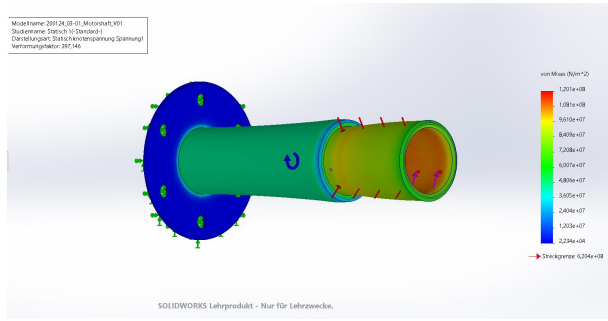
\includegraphics[width=0.6\textwidth]{texfiles/mech/eimg/propulsion/picture_simulation_motorshaft}
\caption{Finite Element Method (FEM) simulation results for the Motor shaft}
\label{fig:motorshaft_simulation}
\end{figure}

The result of simulating the pressfitted gearshaft gives a maximum stress of \(286.1 \, \text{MN/m}^2\) and thus a safety factor of \(2.027\) and is therefore stable enough for its area of application.

\begin{figure}[H]
\centering
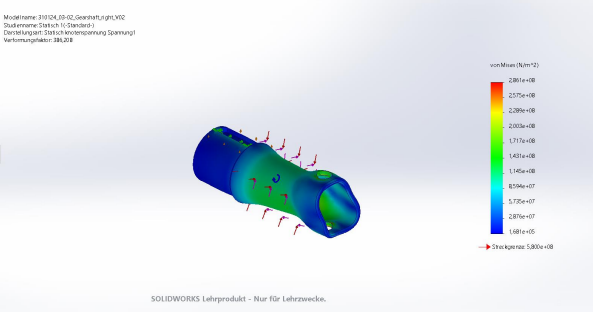
\includegraphics[width=0.6\textwidth]{texfiles/mech/eimg/propulsion/picture_simulation_gearshaft_right}
\caption{Finite Element Method (FEM) simulation results for the pressfitted Gearshaft}
\label{fig:gearshaft_simulation}
\end{figure}

The result of simulating the bolted gearshaft gives a maximum stress of \(288.1 \, \text{MN/m}^2\) and thus a safety factor of \(2.013\) and is therefore stable enough for its area of application.

\begin{figure}[H]
\centering
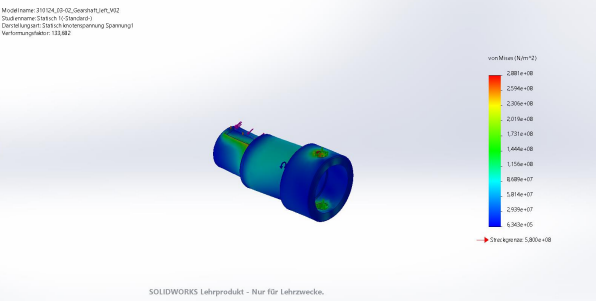
\includegraphics[width=0.6\textwidth]{texfiles/mech/eimg/propulsion/picture_simulation_gearshaft_left}
\caption{Finite Element Method (FEM) simulation results for the bolted Gearshaft}
\label{fig:gearshaft_simulation}
\end{figure}

The result of simulating the wheelshaft gives a maximum stress of \(284 \, \text{MN/m}^2\) and thus a safety factor of \(2.042\) and is therefore stable enough for its area of application. As this part is identical on both sides of the pod and has to withstand the same forces, we are only showing a single simulation here.

\begin{figure}[ht]
\centering
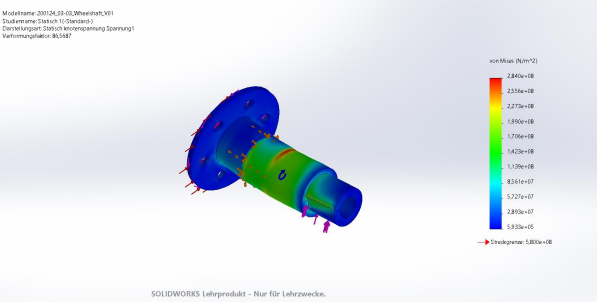
\includegraphics[width=0.6\textwidth]{texfiles/mech/eimg/propulsion/picture_simulation_wheelshaft}
\caption{Finite Element Method (FEM) simulation results for the wheelshaft}
\label{fig:wheelshaft_simulation}
\end{figure}

The result of simulating the wheel gives a maximum stress of \(19.89 \, \text{MN/m}^2\) and while we manufacture this of a Aluminum 6061 compuond, a safety factor of \(2.772\) and is therefore stable enough for its area of application. As this part is identical on both sides of the pod and has to withstand the same forces, we are only showing a single simulation here.

\begin{figure}[H]
\centering
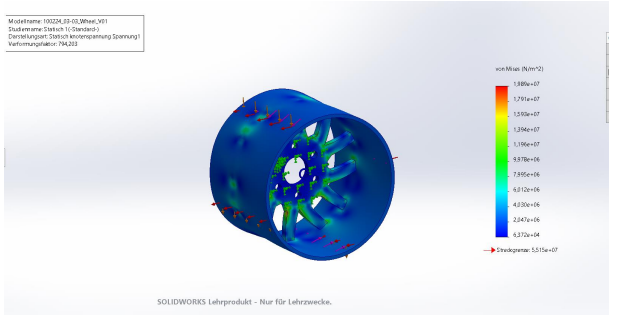
\includegraphics[width=0.6\textwidth]{texfiles/mech/eimg/propulsion/picture_simulation_wheel}
\caption{Finite Element Method (FEM) simulation results for the wheels}
\label{fig:wheel_simulation}
\end{figure}

The result of simulating the motorbracket gives a maximum stress of \(XX \, \text{N/m}^2\) and thus a safety factor of \(XX\) and is therefore stable enough for its area of application. As this part is identical on both sides of the pod and has to withstand the same forces, we are only showing a single simulation here.

%\begin{figure}[H]
%\centering
%\includegraphics[width=0.6\textwidth]{texfiles/mech/eimg/propulsion/picture_simulation_motorbracket}
%\caption{Finite Element Method (FEM) simulation results for the motorbracket}
%\label{fig:motorbracket_simulation}
%\end{figure}

The result of simulating the motorshaftbracket gives a maximum stress of \(XX \, \text{N/m}^2\) and thus a safety factor of \(XX\) and is therefore stable enough for its area of application. As this part is identical on both sides of the pod and has to withstand the same forces, we are only showing a single simulation here.

%\begin{figure}[H]
%\centering
%\includegraphics[width=0.6\textwidth]{texfiles/mech/eimg/propulsion/picture_simulation_motorshaftbracket}
%\caption{Finite Element Method (FEM) simulation results for the motorshaftbracket}
%\label{fig:motorshaftbracket_simulation}
%\end{figure}

The result of simulating the bearinghouse gives a maximum stress of \(XX \, \text{N/m}^2\) and thus a safety factor of \(XX\) and is therefore stable enough for its area of application. As this part is identical on both sides of the pod and has to withstand the same forces, we are only showing a single simulation here. As this part is identical on both sides of the pod and has to withstand the same forces, we are only showing a single simulation here.

%\begin{figure}[H]
%\centering
%\includegraphics[width=0.6\textwidth]{texfiles/mech/eimg/propulsion/picture_simulation_bearinghouse}
%\caption{Finite Element Method (FEM) simulation results for the bearinghouses}
%\label{fig:bearinghouse_simulation}
%\end{figure}

The result of simulating the bearingbracket gives a maximum stress of \(XX \, \text{N/m}^2\) and thus a safety factor of \(XX\) and is therefore stable enough for its area of application. As this part is identical on both sides of the pod and has to withstand the same forces, we are only showing a single simulation here. As this part is identical on both sides of the pod and has to withstand the same forces, we are only showing a single simulation here.

%\begin{figure}[H]
%\centering
%\includegraphics[width=0.6\textwidth]{texfiles/mech/eimg/propulsion/picture_simulation_bearingbracket}
%\caption{Finite Element Method (FEM) simulation results for the bearingbrackets}
%\label{fig:bearingbracket_simulation}
%\end{figure}

\subsubsection{Mesh and Boundary Conditions}
For meshing and specify all required parameters for a successful simulation, we used the standardsettings of Solidworks.

\subsection{Manufacturing Process}
\begin{table}[H]
\centering
\begin{adjustbox}{width=\textwidth}
\begin{tabular}{|>{\bfseries}m{5cm}|m{1,5cm}|m{8cm}|}
\hline
Component & Number & Required procedures \\
\hline
Motorshaft & x1 & latheturning, milling \\
\hline
Gearshaft Pressfitted & x1 & latheturning, milling, hydraulic pressing \\
\hline
Gearshaft bolted & x1 & latheturning, milling \\
\hline
Wheelshaft & x2 & latheturning, milling \\
\hline
Wheel & x2 & latheturning, milling \\
\hline
Motorbracket & x1 & lasercutting  \\
\hline
Wheelshaftbracket & x1 & lasercutting  \\
\hline
Bearinghouse & x2 & lasercutting  \\
\hline
Bearingbracket & x2 & lasercutting, welding \\
\hline
\end{tabular}
\end{adjustbox}
\caption{Components and Manufacturing Details}
\label{table:components}
\end{table}

\subsection{Integration process}

\subsubsection{Assembling}
Describe how the parts will be assembled, including integration into subordinate structures/systems if applicable.

\subsubsection{Assembly interaction}
If applicable, describe how the assembly interacts with other assemblies.



\subsection{Safety considerations }
(a) Discuss the safety factor applied to structural elements. \\
(b) If applicable, discuss the safety factor applied to the demagnetization of permanent mag-
nets.\\
(c) If applicable, discuss high voltage safety considerations for the motor.\\
(d) Discuss worst-case scenarios (e.g., worst-case braking deceleration) and what you plan
to do to avoid or contain them.\\

\subsection{FMEA}
\textbf{WILL BE DONE BY PM}

\subsubsection{Expected Outcomes}
Detail the anticipated results from the testing and validation processes.

\subsubsection{Risk Mitigation}
Discuss the potential risks associated with the system and how they will be mitigated.

\paragraph{Impact Resistance}
Detail a contingency plan in case the system does not perform as expected.


\subsection{Testing}
Provide a test plan including setup, procedure, and expected outcomes.
Outline which factors are critical to success and how they will be validated.


\subsection{Full-scale adaptation}
- Funktioniert wie herkömmliche Eisenbahn
- Für die Beschleunigung im Full scale möglich
- Sobald der Pod mit levitation anfängt, werden die Reifen angehoben, und das derzeitige propulsion system abgeschaltet

\subsection{References}

\begin{figure}[H]
\centering
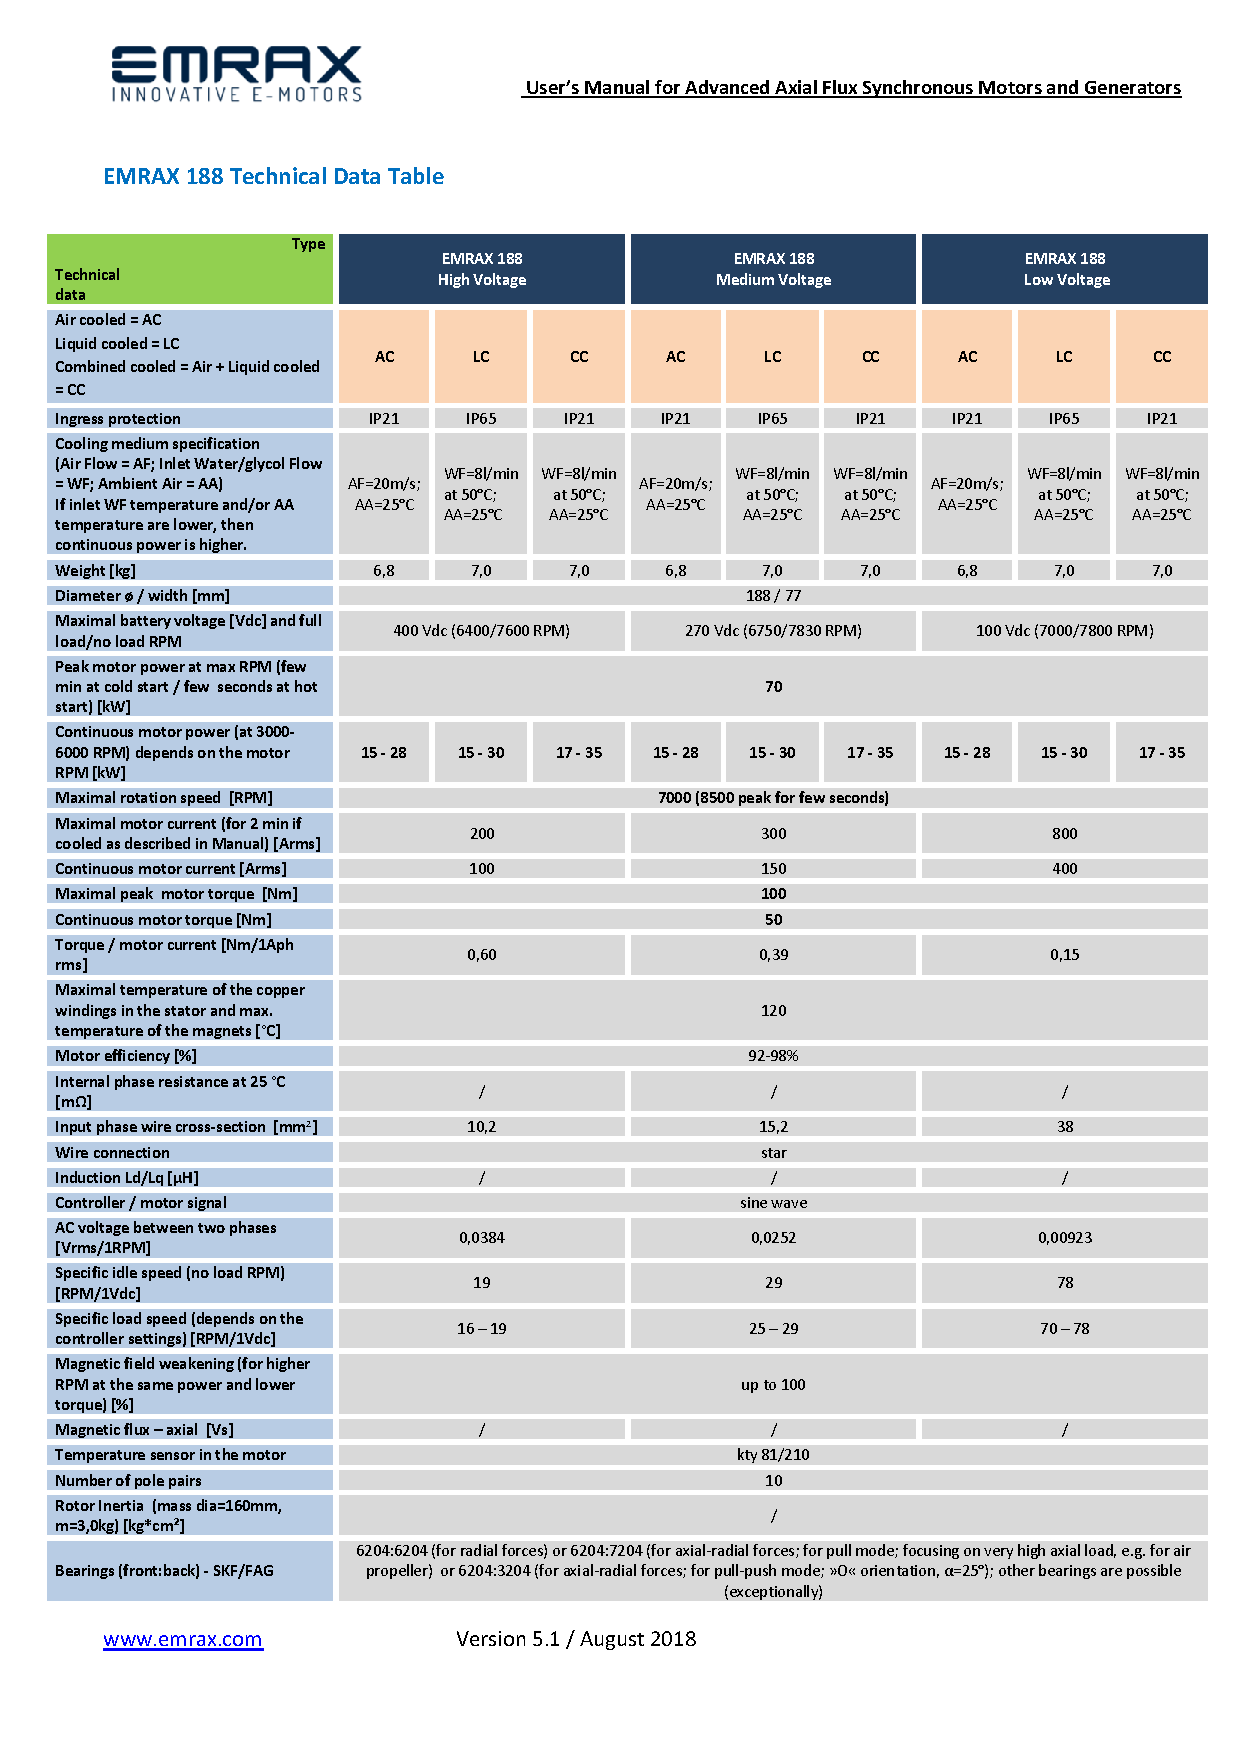
\includegraphics[width=0.9\textwidth]{texfiles/mech/eimg/propulsion/table_motor}
\caption{Motor Specifications}
\label{tab: Motor Specifications}
\end{figure}
 \newpage



\section{Cooling System} 
\subsection{Overview}
\subsubsection{Requirements and Constraints}
The cooling system plays a pivotal role in keeping the motor, battery, and traction controller within safe temperature limits. Overheating can lead to reduced efficiency and potentially shorten the lifespan of these components. For instance, excessive heat could cause bearings to wear out faster, damage motor windings, and even demagnetize permanent magnets. Given the hyperloop's low-pressure environment, we must think beyond standard air cooling methods. Consequently, the exploration of alternative cooling techniques, such as liquid cooling, cooling with the Phase Changing Materials are becoming imperative for ensuring the system's reliability and efficiency.

\subsubsection{Estimated Cost and Part List}
The total estimated manufacturing cost for the cooling system is approximately 1200 Euros, considering the primary components outlined in the table. Despite its comprehensive functionality, the system maintains a relatively lightweight and compact profile, comprising only a select few components. This cost-effective design approach ensures efficient performance without compromising on reliability or functionality.


\autoref{table:components}
\begin{table} [H]
\centering
\caption{Components and Manufacturing Details}
\label{table:components}
\begin{adjustbox}{width=\textwidth,center}
\begin{tabular}{|>{\bfseries}m{2.9cm}|m{2.4cm}|m{1.7cm}|m{2.5cm}|m{2.2cm}|m{2.6cm}|m{2.2cm}|}
\hline
Component & Number & Mass [kg] & Size [mm] & Material & Manufacturing process & In-house/ Outsourced \\
\hline
Heat Exchanger & x1 & 1.1 & 100 x120 x100 & Aluminum & LPBF Printing & in-house \\
Drain Valve & x1 & 0.02 & M8 & Aluminum & Latheturning & in-house \\
PCM & x1.75 [liters] & 2 & - & PCM & - & outsourced \\
Deionized Water & x3 [liters] & 3 & - & Water & - & outsourced \\
Coolant Pump & x1 &1.2 & - & - & - & outsourced \\
Filter &x1 & 0.1 & - & - & - &outsourced \\
Coolant Temperature Sensor & x2 & 0.2 & - & - & - & outsourced \\
Surface Temperature Sensor & x3 & 0.2 & - & - & - & outsourced \\
Flow Meter & x1 & 0.1 & - & - & - & outsourced \\
Pressure Sensor & x4 & 0.1 & - & - & - & outsourced \\
Piping & x5 [meters] & 0.9 &  10 x 16& - & - & outsourced \\
Piping & x2 [meters] & 0.4 & 20 x 26 & - & - & outsourced \\
Tank & x1 & 0.2 & 138 x 160 & - & - & outsourced \\

Fittings & x15 & - & - & - & - & outsourced \\
\hline
\end{tabular}
\end{adjustbox}
\end{table}


\subsection{Objectives, Design process, and Cooling Requirements}
\autoref{fig:Cooling system}
\begin{figure}[ht]
  \centering
  \subfloat[Front view of the pod]{
    \centering
    \includegraphics[width=0.5\linewidth]{texfiles/mech/eimg/cooling/placeholder}
    \label{fig:Front view}
  }
  \subfloat[Top view of the pod]{
    \centering
    \includegraphics[width=0.5\linewidth]{texfiles/mech/eimg/cooling/placeholder}
    \label{fig:Top view}
  }
  \caption{Placement of the Cooling system}
  \label{fig:Cooling system}
\end{figure}


\subsubsection{ Motor}
The EMRAX motor is required to operate within a temperature range of -40°C to 120°C for both the copper windings and magnets. To safeguard against overload, a temperature sensor is integrated into the motor and must be linked to the controller. If the temperature surpasses the permissible limit, the controller adjusts the motor's current output to lower levels until the temperature stabilise within the acceptable range, with a worst-case motor efficiency of 92\%, approximately 4.8 kW of heat is generated during operation.

The manufacturer recommends a coolant flow rate of 6 to 8 litres per minute, with the coolant maintained at a maximum temperature of 50°C when entering the motor. Additionally, ambient air temperature surrounding the motor should ideally be 25°C or lower. [Ref - Product Spec Emrax Motor]


\subsubsection{ Traction Controller}

According to the product specification, the maximum permissible temperature for the traction controller is 150°C. However, to guarantee peak performance and longevity, it's essential to maintain temperatures below 90°C. After assessing the operating current and internal resistance, the estimated heat generation was calculated to be 0.56 kW. Through heat transfer calculations from the power module baseplate, equipped with fins, to the coolant, a water flow rate of 0.7 litres per minute was determined necessary to sustain the traction controller's temperature at 90°C.This ensures optimal cooling performance and contributes to the longevity and efficiency of the entire cooling system.
\subsubsection{ Battery}
The battery system within the hyperloop pod generates approximately 3.84 kW of heat during operation. This heat generation is primarily due to internal resistance within the battery cells as electrical energy is converted into usable power. To maintain safe and efficient operation, it is imperative to ensure that the temperature of the battery remains below 75°C.

When a battery operates at elevated temperatures, several detrimental effects may occur. High temperatures can accelerate the degradation of battery components, including the electrolyte and electrode materials, leading to reduced battery capacity and lifespan. Additionally, overheating increases the risk of thermal runaway, a phenomenon where the battery temperature rapidly increases, potentially resulting in fire or explosion.


\subsubsection{Cooling Requirements and Strategies}
To mitigate these risks and ensure the longevity and safety of the battery system, effective cooling strategies are essential. This includes implementing cooling systems, such as liquid cooling or cooling plates, to dissipate the heat generated by the battery during operation.

To ensure optimal cooling for all three vital components, the system necessitates a total coolant volume of 1 liters of de-ionised water. This calculation factors in the total heat generation (9.2 kW), the duration of a single run at the European Hyperloop Week Competition (20 seconds), and a safety factor of 3 (total time 60 seconds). After 60 seconds of operation, the maximum temperature of the 3 liters of coolant reaches approximately 66.5°C, well below the specified temperature limits. Further analysis during testing phase will provide valuable insights into coolant temperature changes and component temperatures.

To enhance the cooling performance of the cooling System, a refined hardware architecture will be implemented. Temperature levels play a critical role in determining the durability and efficiency of the motor, battery, and traction controller within the hyperloop pod. Elevated temperatures can adversely affect various components, including bearings, motor windings, and permanent magnets, potentially leading to demagnetisation. Therefore, prioritising the enhancement of cooling systems is essential for achieving significant long-term cost savings and improved performance. Given the impracticality of air cooling in the low-pressure hyperloop tube environment, alternative approaches such as liquid cooling and the use of Phase changing materials must be explored.

\subsubsection{Hardware Architecture for Enhanced Cooling}

As illustrated in  figure ~\ref{fig:schematic}, cold water stored at room temperature (approximately 20-25°C) will undergo filtration and then be pumped into the water jackets of the motor, traction controller, and battery in a closed-loop configuration, with a flow rate ranging from 8 to 12 liters per minute. Continuous monitoring of the coolant, motor, traction controller, and battery temperatures will be conducted. Should the temperature of any component exceed the specified limit, the control system will promptly deactivate the pod's drive motor.

Given the absence of heat transfer with the atmosphere during operation, the coolant temperature will gradually increase. Consequently, it's imperative that the coolant within the system remains below the temperature limits of each component. Cooling down the coolant prior to the pod's subsequent operation will be necessary.s
Pressure sensors have been strategically positioned at designated locations, as depicted in the diagram, to accurately gauge pressure drops across the water jackets during the testing phase. This data will be instrumental in fine-tuning the system's performance and ensuring optimal cooling efficiency.

\subsection{Appearance and Integration}
\subsubsection{Coolant }
Deionized water has been selected as the primary coolant for the system due to its low electrical conductivity. This choice is paramount in minimising the potential adverse effects of coolant leaks on the pod's electronic components. Although glycol is a common coolant choice in many cooling systems, it is not utilized in this particular system. This decision is attributed to the fact that the operating temperatures within the system consistently remain well above the freezing point of water, rendering glycol unnecessary.
\subsubsection{Coolant Pump}
During the testing phase, the Rheinmetall WUP 25 pump will serve as the primary pump for the cooling system. Although typically employed in the realm of combustion engines and vehicle climate control systems, the WUP 25 pump demonstrates versatility by effectively handling various cooling tasks, including cooling DC/DC converters, batteries, electric motors, and power electronics. Its compact design allows for installation in constrained spaces, and it offers a range of hydraulic and electrical interfaces to suit diverse applications. Equipped with a control and diagnostic pin, the WUP 25 pump facilitates speed control via a PWM input signal [Ref = Product Data Sheet WUP 25]. 

To ensure optimal performance, the pump will be mounted at a mid-level position within the cooling circuit. This strategic placement helps prevent the formation of air traps (if mounted at the highest position) and minimizes the risk of debris accumulation within the pump (if mounted at the lowest position) [Ref = Product Data Sheet WUP 25]. However, due to the current uncertainty regarding the pressure drop in the system, it may be necessary to explore alternative pump options or implement a multi-stage pump system (in series) alongside the existing model. The exact pressure drop across the water jackets will be determined through rigorous testing
\begin{figure}[ht]
  \centering
  \includegraphics[width=0.5\linewidth]{texfiles/mech/eimg/cooling/placeholder}
  \caption{Coolant pump}
  \label{fig:Coolant Pump}
\end{figure}

\subsubsection{Coolant Storage Tank}
The cooling system is designed with consideration for the realistic scenario of the pod traveling through a low-pressure tube (near vacuum), limiting heat exchange with the atmosphere. The coolant in the circuit absorbs heat from the motor, battery, and traction controller, causing an increase in coolant temperature over time. The current design ensures sufficient coolant storage to keep all components well below the required maximum operating temperature.

For the hyperloop pod slated for participation in the European Hyperloop Week, a typical vehicle coolant tank with a capacity of 1 liter has been deemed adequate. This capacity aligns with the demands of the pod's cooling requirements, guaranteeing optimal performance throughout its operation.
\begin{figure}[ht]
  \centering
  \includegraphics[width=0.5\linewidth]{texfiles/mech/eimg/cooling/placeholder}
  \caption{Coolant tank}
  \label{fig:Coolant tank}
\end{figure}

\subsubsection{Water Jackets}
The water jacket for the motor will be provided by the motor manufacturer, ensuring compatibility and optimal performance. For the water jackets of the traction controller and battery, custom fabrication will be undertaken based on the recommendations provided by their respective manufacturers. This approach guarantees that each component receives tailored cooling solutions to meet its specific requirements and operating conditions.

\subsubsection{Piping}
Two piping options are under consideration.
 i) CPVC pipes, chosen for their resistance to high temperatures, scaling, durability, low cost, and ease of installation. The specific piping route is yet to be finalized , but the total length is estimated to be around 6 meters. 
ii) The potential use of soft tubing is also being explored.

\subsection{Heat Exchanger}
\subsubsection{Role and Benefits in the cooling System}
In the context of the cooling system described for the hyperloop pod, a heat exchanger would play a crucial role in transferring heat between the coolant circulating within the closed-loop system and the surrounding environment. As the coolant circulates through the system, it absorbs heat from the motor, battery, and traction controller, thereby increasing in temperature. Since the hyperloop pod operates in a low-pressure tube with limited heat exchange with the atmosphere, the heat exchanger facilitates the dissipation of heat even in this constrained environment.

\begin{figure}[ht]
  \centering
  \subfloat[Closed View]{
    \centering
    \includegraphics[width=0.5\linewidth]{texfiles/mech/eimg/cooling/placeholder}
    \label{fig:HE Closed view}
  }
  \subfloat[Open View]{
    \centering
    \includegraphics[width=0.5\linewidth]{texfiles/mech/eimg/cooling/placeholder}
    \label{fig:HE Open view}
  }
  \caption{Gyroid Heat Exchanger}
  \label{fig:HE}
\end{figure}


\subsubsection{Use of Phase Change Materials (PCMs)}
Introducing the heat exchanger utilizing phase change materials (PCMs) into the cooling system for the hyperloop pod would offer several advantages and could enhance its performance in specific scenarios, incorporating a heat exchanger with the use of phase changing material serves several important purposes:

\begin{itemize}
  \item \textbf{Enhanced Heat Absorption and Release:} The PCM, such as stearic acid, can absorb and release a significant amount of heat during its phase transition from solid to liquid and vice versa. Integrating a heat exchanger with PCM allows for efficient absorption of excess heat generated by components like the motor, traction controller, and battery.
  \item \textbf{Temperature Regulation:} By absorbing excess heat from critical components, the heat exchanger helps regulate their temperatures within the specified operating ranges. This prevents overheating, which can lead to performance degradation or damage to components.
  \item \textbf{Thermal Energy Storage:} The PCM's ability to store thermal energy during its phase change enables the system to store heat when temperatures are within acceptable limits and release it when needed to maintain optimal operating conditions. This helps in managing transient heat loads and stabilizing temperatures over time.
  \item \textbf{Reduced Coolant Temperature:} By utilizing the PCM's heat absorption capacity, the heat exchanger can lower the temperature of the coolant circulating in the system. This ensures that the coolant remains within acceptable temperature limits, contributing to the overall effectiveness of the cooling system.
  \item \textbf{Increased Efficiency:} Integrating a heat exchanger with PCM can improve the overall efficiency of the cooling system by maximizing heat transfer capabilities and reducing the reliance on conventional cooling methods alone.
  \item \textbf{Extended Operating Time:} The thermal energy stored in the PCM can be utilized to extend the operating time of the system before coolant temperature rises beyond acceptable levels. This can be particularly beneficial during transient operating conditions or in the event of temporary power interruptions.
\end{itemize}

Overall, incorporating a heat exchanger with the use of phase changing material adds an additional layer of heat management capability to your cooling system, contributing to improved performance, efficiency, and reliability in the hyperloop pod environment.


\subsubsection{Stearic Acid}

Stearic acid stands out as a highly versatile phase change material (PCM) deployed across diverse applications. Its unique characteristic of transitioning from solid to liquid state at a precise temperature renders it exceptionally suitable for thermal energy storage purposes. Through this phase transition, stearic acid exhibits remarkable heat absorption and release capabilities, making it a valuable asset in scenarios demanding efficient temperature regulation and thermal energy management. Commonly found in applications ranging from building insulation to specialized temperature control systems, stearic acid's efficacy as a PCM underscores its widespread industrial utility.

\paragraph{Stearic Acid}
Stearic acid is a saturated fatty acid with the chemical formula \( C_{18}H_{36}O_2 \). It is a long-chain carboxylic acid, meaning it has 18 carbon atoms in its hydrocarbon chain and a carboxyl group (COOH) at one end. Here are some key properties and uses of stearic acid:

\subparagraph{Physical Properties:}
\begin{itemize}
  \item Melting Point: Stearic acid is a solid at room temperature and has a melting point of around \( 69-70 \) degrees Celsius (\( 156-158 \) degrees Fahrenheit).
  \item Appearance: It is a white, waxy solid with a characteristic fatty odor.
\end{itemize}

\subparagraph{Chemical Properties:}
\begin{itemize}
  \item Structure: Stearic acid has a straight-chain structure with 18 carbon atoms, making it a saturated fatty acid. Hydrophobic: Like other fatty acids, stearic acid is hydrophobic, meaning it repels water.
\end{itemize}

In summary, stearic acid is a versatile compound with various industrial applications, and its phase change properties make it useful in thermal energy storage applications as well.

\subsection{Calculations and Simulations}

\textbf{WILL BE ADDED SOON (Dino)}
\subsection{Safety Measures}
Given the close integration of the cooling system with the electronic systems, the primary risk is a coolant leak that could potentially damage electronic components. Preventive measures are outlined in the table below, and deionised water is chosen as the preferred coolant due to its low conductivity.
\subsubsection{Potential Failure Modes and Risk Mitigation-}
\begin{itemize}
  \item \textbf{Coolant Leaks}
    \begin{itemize}
      \item Effect of Failure: Damage Electronic components
      \item Root Cause: Poor sealing at pipe joints
      \item Risk Mitigation Strategy: Maintain the correct coolant level, avoid overfilling the tank, sealing pipes with hose clamps and use deionized water as a coolant.
    \end{itemize}
  \item \textbf{Temperature of Critical component rises above rated temperature}
    \begin{itemize}
      \item Effect of Failure: Damage Component
      \item Root Cause: Insufficient cooling due to prolonged operation
      \item Risk Mitigation Strategy: Implement a control system to halt the motor and by installing two temperature sensors if temperatures exceed prescribed limits for the motor, battery, or traction controller.
    \end{itemize}
  \item \textbf{Temperature of Critical component rises above rated temperature}
    \begin{itemize}
      \item Effect of Failure: Coolant Leaks
      \item Root Cause: Insufficient cooling due to air traps or exceeding defined operation time
      \item Risk Mitigation Strategy: Position of the system including heat exchanger is placed at the front of the pod, in order to purge air after refilling, and adhere to defined operation times.
    \end{itemize}
  \item \textbf{Blocks in piping}
    \begin{itemize}
      \item Effect of Failure: Insufficient cooling and damage to components
      \item Root Cause: Foreign particles/debris
      \item Risk Mitigation Strategy: Introduce filters in the piping system and conduct regular cleaning maintenance.
    \end{itemize}
\end{itemize}


\subsubsection{FMEA analysis}

\textbf{Failure Mode: Coolant Leaks}
\begin{itemize}
  \item Effects of Failure: Damage to Electronic components
  \item Severity: High
  \item Causes of Failure: Poor sealing at pipe joints
  \item Occurrence: Medium
  \item Current Controls: Regular inspection for leaks, pressure testing of the system
  \item Detection: Visual inspection, pressure sensors
  \item Risk Priority Number (RPN): Severity * Occurrence * Detection
  \item Recommended Actions: Improve seal quality, implement redundant sealing, increase inspection frequency
  \item Responsibility: Mechanical Team
  \item Actions Taken: Upgraded sealing materials, added secondary containment
  \item Revised RPN: After action taken
\end{itemize}

\textbf{Failure Mode: Temperature of Critical Component Rises Above Rated Temperature (First Instance)}
\begin{itemize}
  \item Effects of Failure: Damage to Component
  \item Severity: High
  \item Causes of Failure: Insufficient cooling due to prolonged operation
  \item Occurrence: High
  \item Current Controls: Thermal cutoff switches, temperature monitoring
  \item Detection: Thermal sensors with automated system feedback
  \item Risk Priority Number (RPN): Severity * Occurrence * Detection
  \item Recommended Actions: Implement more efficient cooling mechanisms, revise operational protocols to prevent prolonged operation without cooling
  \item Responsibility: Electrical Team
  \item Actions Taken: Included additional cooling systems, adjusted operational limits
  \item Revised RPN: After action taken
\end{itemize}

\textbf{Failure Mode: Temperature of Critical Component Rises Above Rated Temperature (Second Instance)}
\begin{itemize}
  \item Effects of Failure: Coolant Leaks
  \item Severity: High
  \item Causes of Failure: Insufficient cooling due to air traps or exceeding defined operation time
  \item Occurrence: Medium
  \item Current Controls: Coolant system design to avoid air traps, operational time limits
  \item Detection: Temperature and flow sensors
  \item Risk Priority Number (RPN): Severity * Occurrence * Detection
  \item Recommended Actions: Redesign of the coolant flow paths to eliminate air traps, strict adherence to operational time limits
  \item Responsibility: Design Team
  \item Actions Taken: Coolant flow paths optimized, operational procedures updated
  \item Revised RPN: After action taken
\end{itemize}

\textbf{Failure Mode: Blocks in Piping}
\begin{itemize}
  \item Effects of Failure: Insufficient cooling and damage to components
  \item Severity: Medium
  \item Causes of Failure: Foreign particles/debris
  \item Occurrence: Low
  \item Current Controls: Filtration systems, preventive maintenance schedules
  \item Detection: Flow rate monitoring, pressure differential sensors
  \item Risk Priority Number (RPN): Severity * Occurrence * Detection
  \item Recommended Actions: Improve filtration system, implement more rigorous maintenance and cleaning schedules
  \item Responsibility: Maintenance Team
  \item Actions Taken: Upgraded filters, more frequent cleaning
  \item Revised RPN: After action taken
\end{itemize}
\subsubsection{References}

\begin{figure}[ht]
  \centering
  \includegraphics[width=\linewidth]{texfiles/mech/eimg/cooling/placeholder}
  \caption{Flowchart of the system}
  \label{fig:schematic}
\end{figure}

%add schematic




\newpage
